\documentclass[journal]{IEEEtran}

\usepackage{cite}
\usepackage{amsmath,amssymb,amsfonts}
\usepackage{algorithmic}
\usepackage{graphicx}
\usepackage{textcomp}
\usepackage{xcolor}
\usepackage{booktabs}
\usepackage{array}
\usepackage{url}
\usepackage{microtype}
\usepackage{multirow}
\usepackage{balance}
\usepackage{lettrine}
\usepackage{fancyhdr}

% Page style: page number top-right, no running header text
\pagestyle{fancy}
\fancyhf{}
\fancyhead[R]{\thepage}
\renewcommand{\headrulewidth}{0pt}
\fancypagestyle{plain}{%
  \fancyhf{}
  \fancyhead[R]{\thepage}
  \renewcommand{\headrulewidth}{0pt}
}

% Float placement
\renewcommand{\topfraction}{0.95}
\renewcommand{\bottomfraction}{0.85}
\renewcommand{\textfraction}{0.05}
\renewcommand{\floatpagefraction}{0.80}

\hyphenation{net-work semi-conduc-tor shadhin-ai packet-drop through-put}

\begin{document}

\title{Autonomous Post-Quantum Cyber Defense Agent (ASM-Shadhin-AI):
  Sovereign Line-Rate Intrusion Defense via Kernel-eBPF and Local-LLM}

\author{A~S~M~Hossain~Mahmud~(Shadhin),~\textit{Department~of~CSE,~Bangladesh~Army~University~of~Science~and~Technology~(BAUST),~Saidpur~5310,~Bangladesh}}

\maketitle
\thispagestyle{fancy}

% =============================================================================
\begin{abstract}
% =============================================================================
Modern network perimeters face a fundamental trade-off between inspection
depth, inline latency, and operational data sovereignty. Conventional
user-space intrusion-prevention systems (e.g., Snort~3.x, Suricata~7.x)
operate via packet-capture interfaces, incurring socket-buffer allocation
penalties, soft-interrupt saturation, and $180$--$800\,\mu\text{s}$
queuing latencies that cause measurable packet drops under multi-gigabit
loads. Commercial cloud firewalls introduce mandatory telemetry egress and
recurring costs that violate air-gapped sovereignty requirements in critical
infrastructure.

This paper presents \textbf{ASM-Shadhin-AI}, an open, fully sovereign,
line-rate intrusion-mitigation and cognitive-defense architecture uniting
in-kernel fast-path execution with asynchronous edge intelligence and
post-quantum cryptographic resilience. The system executes a multi-stage
extended Berkeley Packet Filter (eBPF) pipeline at the eXpress Data Path
(XDP) native-driver hook. CIDR blocklist lookups are implemented via
\texttt{BPF\_MAP\_TYPE\_LPM\_TRIE} (Longest Prefix Match), providing
$O(\log N)$ worst-case complexity with kernel-JIT-compiled branch elimination
reducing average lookup latency to approximately $64\,\text{ns}$ under the
tested workload. Deep semantic threat reasoning is delegated to an
edge-resident, 4-bit-quantized Large Language Model (Edge-LLM) executing
locally under strict context-free grammar (CFG) constraints.

ASM-Shadhin-AI integrates proactive Moving Target Defense (MTD) using
HMAC-SHA256 synchronized port hopping, with epoch keys established via NIST
FIPS~203 (ML-KEM-1024) and authenticated via FIPS~204 (ML-DSA-65).

Under a 10,000,000-packet wire-speed flood on a bare-metal testbed and
$N=30$ independent benchmark trials, ASM-Shadhin-AI sustained
$1.495 \pm 0.015\,\text{Mpps}$ ($1.18\,\text{Gbps}$) throughput with
$0.0000\%$ packet drop (under the tested load) and $26.2 \pm 0.6\%$ mean CPU
utilization. Mean per-packet in-kernel processing latency was
$0.126 \pm 0.007\,\mu\text{s}$, with an observed XDP-pipeline stage peak of
$0.33\,\mu\text{s}$. Compared with Linux Netfilter (mean
$26.49 \pm 1.65\,\mu\text{s}$), this represents a
$5.30\times$ throughput advantage and a $\approx\!210\times$ latency reduction
($p < 10^{-15}$, Welch's two-sample \textit{t}-test, Welch--Satterthwaite $\mathit{df} \approx 39.1$,
Cohen's $d = 108.2$, 95\% CI for throughput: $[1.489,\,1.500]\,\text{Mpps}$).
DPDK achieves higher raw forwarding throughput ($3.798\,\text{Mpps}$) under the
tested single-core configuration but requires $100\%$ dedicated CPU core busy-polling.
In end-to-end subsystem ablation, ASM-Shadhin-AI achieved 98.64\% evasion recall.
The Edge-LLM daemon was evaluated separately across 50 labeled threat scenarios,
achieving 96.0\% overall accuracy (48/50). Over the 40 non-adversarial
classification scenarios (UNSW-NB15 and CSE-CIC-IDS2018 malicious plus benign
traffic), precision, recall, and F1-score were each 0.967. All 10 adversarial
context-free grammar (CFG)-stress scenarios produced valid, executable
directives, confirming CFG-constrained decoding robustness under the tested inputs.
\end{abstract}

\begin{IEEEkeywords}
Extended Berkeley Packet Filter (eBPF), eXpress Data Path (XDP),
Autonomous Cyber Defense, Edge Large Language Model (Edge-LLM),
Post-Quantum Cryptography, ML-KEM-1024, ML-DSA-65, Moving Target Defense,
Shannon Entropy, Line-Rate Mitigation, Air-Gapped Security.
\end{IEEEkeywords}

\IEEEpeerreviewmaketitle

% =============================================================================
\section{Introduction}
% =============================================================================
\lettrine[lines=3,loversize=0.08,findent=2pt,nindent=0pt]{P}{rotecting} enterprise
and critical-infrastructure network perimeters against modern cyber threats requires
reconciling two conflicting operational demands: line-rate packet forwarding at sub-microsecond
latencies, and deep semantic inspection capable of detecting polymorphic attacks.
Contemporary adversaries deploy multi-vector strategies---combining multi-gigabit volumetric
SYN/UDP floods, evasive low-and-slow reconnaissance sweeps, and encrypted command-and-control
(C2) beacons over TLS~1.3---to bypass conventional perimeter
controls~\cite{sarhan2022standard,mirsky2018kitsune}.

Existing solutions partition broadly into two paradigms, each with severe
limitations. Open-source Intrusion Detection and Prevention Systems (IDS/IPS)
such as Snort~3.x and Suricata~7.x operate in user-space via packet-capture
interfaces (\texttt{AF\_PACKET}, \texttt{DAQ})~\cite{roesch1999snort}. Under
gigabit traffic loads, the associated kernel-to-user copy overhead and
rule-evaluation latency ($180$--$800\,\mu\text{s}$) induce measurable packet
drops, enabling evasion attacks. Detection mechanisms rely primarily on
syntactic pattern matching, leaving systems vulnerable to polymorphic variants
and zero-day exploits.

Commercial Next-Generation Firewalls (e.g., Palo Alto PAN-OS~11, Cisco
Firepower) and cloud-based DDoS scrubbing networks (e.g., Cloudflare Magic
Transit) provide deeper inspection but introduce three disqualifying
trade-offs: \emph{(1)~Telemetry Leakage}: network metadata and decrypted
packet payloads are transmitted to third-party cloud infrastructure, violating
data-sovereignty mandates in defense and classified environments;
\emph{(2)~Operational Dependency}: defense perimeters degrade in air-gapped
or degraded network settings; and \emph{(3)~Financial Overhead}: recurring
subscription licensing (\$40{,}000--\$200{,}000 annually) places
enterprise-grade defense out of reach for resource-constrained institutions.

To address this trilemma, we present \textbf{ASM-Shadhin-AI}, an open-source,
fully sovereign network defense architecture integrating wire-speed in-kernel
mitigation with local, offline AI-driven threat reasoning and post-quantum
cryptographic resilience.

\subsection{Research Contributions}
This paper makes five primary technical contributions:
\begin{enumerate}
  \item \textbf{Sub-Microsecond In-Kernel Fast Data Plane:} We implement an
    eBPF/XDP packet-processing pipeline executing inside the NIC driver callback
    prior to socket-buffer allocation. The pipeline performs LPM trie lookups
    ($O(\log N)$ worst case, ${\approx}64\,\text{ns}$ just-in-time (JIT) compiled
    average) and stateful TCP-flag validation. Measured mean packet processing
    latency is $0.126\,\mu\text{s}$ (observed stage-peak $0.33\,\mu\text{s}$) on
    commodity x86-64 hardware.

  \item \textbf{Air-Gapped Edge-LLM Threat Reasoning:} We decouple deep semantic
    evaluation from the line-rate data path via an asynchronous Edge-LLM triage
    engine. CFG decoding constraints substantially reduce hallucinated outputs and
    syntactic parser crashes. Section~VI provides a rigorous 50-scenario evaluation
    with confusion matrices and confidence intervals.

  \item \textbf{Post-Quantum Moving Target Defense (MTD):} We develop a proactive
    MTD mechanism mutating externally exposed service ports across discrete epochs
    using keyed HMAC-SHA256 pseudo-random permutations. Key establishment is secured
    via NIST FIPS~203 (ML-KEM-1024) and authenticated via FIPS~204 (ML-DSA-65),
    providing indistinguishability under chosen-ciphertext attack (IND-CCA2)
    primitive security against \emph{Store Now, Decrypt Later} (SNDL) attacks under the
    Module Learning With Errors (MLWE) hardness assumption. The measured $1{,}219\times$
    scan-duration increase under an exhaustive Nmap probe configuration is derived in Section~VIII.

  \item \textbf{Zero-Decryption Streaming Entropy Engine:} We implement an inline
    streaming Shannon byte-entropy and inter-arrival timing jitter analyzer
    detecting high-entropy C2 beaconing without Man-in-the-Middle decryption.
    Threshold justification (ROC-curve analysis) and classification performance
    are reported in Section~VI-E.

  \item \textbf{Reproducible Empirical \& Statistical Benchmarking:} Under a
    10,000,000-packet stress flood and $N=30$ independent benchmark runs,
    ASM-Shadhin-AI achieved $1.495 \pm 0.015\,\text{Mpps}$ throughput,
    $0.126 \pm 0.007\,\mu\text{s}$ mean latency, $0.0000\%$ packet loss (under the tested load),
    and $26.2 \pm 0.6\%$ CPU utilization, with a statistically significant $5.30\times$ throughput
    and $\approx\!210\times$ latency improvement over Linux Netfilter
    ($p < 10^{-15}$, Welch's two-sample \textit{t}-test, Welch--Satterthwaite
    $\mathit{df} \approx 39.1$, Cohen's $d = 108.2$ for throughput; $\mathit{df} \approx 29.0$,
    Cohen's $d = 22.7$ for latency; 95\% CI for throughput: $[1.489,\, 1.500]\,\text{Mpps}$).
\end{enumerate}

The remainder of this paper is structured as follows.
Section~II reviews related work and identifies the literature gap.
Section~III establishes the formal threat model and security assumptions.
Section~IV details the system architecture and mathematical foundations.
Section~V describes the eBPF fast data plane, Edge-LLM daemon, and MTD
coordination subsystem. Section~VI presents the empirical testbed and statistical
results. Section~VII provides an ablation study and sensitivity analysis.
Section~VIII discusses defensive deception and tarpit dynamics. Section~IX
examines limitations and future directions. Section~X addresses ethics,
responsible disclosure, and reproducibility, and Section~XI concludes the paper.

% =============================================================================
\section{Related Work \& Literature Gap}
% =============================================================================
\subsection{Programmable Data Planes and In-Kernel Packet Processing}
The performance limitations of user-space packet inspection have long driven
research toward kernel bypass and programmable data planes. Bro (now
Zeek)~\cite{paxson1999bro} and Snort~\cite{roesch1999snort} established
signature-based detection but remain bound to user-space capture interfaces.
Intel Data Plane Development Kit (DPDK) achieved multi-gigabit processing
via poll-mode drivers (PMDs) that bypass the kernel~\cite{miano2018creating},
but requires 100\% dedicated CPU core polling and lacks native OS
security-policy integration.

H{\o}iland-J{\o}rgensen et al.~\cite{hoiland2018express} introduced XDP, enabling
in-kernel verified byte-code execution inside the device driver ring before
\texttt{sk\_buff} creation, achieving line-rate performance comparable to DPDK
while preserving Linux socket abstractions. Subsequent works---Polycube, P4
programmable data planes~\cite{bosshart2014p4}, and edge eBPF/XDP security
architectures~\cite{vieira2020fast,miano2018introducing}---explored programmable
data paths for network defense. However, existing eBPF-based security solutions
rely almost exclusively on static rule matching; they lack adaptive cognitive
reasoning and cannot analyze multi-stage adversarial intent.

\subsection{Machine Learning and Language Models in Network Security}
To detect polymorphic and zero-day threats, research shifted toward ML and deep
neural networks on network telemetry. Mirsky et al.~\cite{mirsky2018kitsune}
proposed Kitsune, an ensemble of autoencoders for online anomaly detection.
Ring et al.~\cite{ring2019survey} surveyed network-based intrusion detection
datasets, highlighting structural evaluation limitations across public benchmarks.
Sarhan et al.~\cite{sarhan2022standard} analyzed CSE-CIC-IDS2018 and UNSW-NB15,
showing that tree-based ensembles achieve high accuracy on static corpora.
Moustafa and Slay~\cite{moustafa2015unsw} introduced UNSW-NB15 spanning nine
attack categories. Sharafaldin et al.~\cite{sharafaldin2018toward} demonstrated
that flow-level features significantly improve detection accuracy.

Graph neural network (GNN)-based approaches such as GRAPHIDS~\cite{zhao2023graphids}
achieve 97.3\% F1-score on provenance graph traces but are incompatible with
real-time per-packet inline enforcement due to $O(|V|^2)$ per-epoch complexity.
Garcia et al.~\cite{garcia2014empirical} showed botnet detection accuracy can
degrade 30--60\% under adversarially crafted perturbations. Anderson and
McGrew~\cite{anderson2016identifying} demonstrated 92.1\% malware classification
via encrypted traffic metadata without payload decryption.

LLMs such as Llama~2~\cite{touvron2023llama} combined with efficient
quantization~\cite{dettmers2023qlora} demonstrated high-quality threat reasoning
capabilities. Bertoli et al.~\cite{bertoli2023ebpf} concluded that combining eBPF
telemetry with AI-based anomaly engines is a promising direction. Nevertheless,
inline LLM deployment at the packet level is impractical due to multi-second
inference latencies. ASM-Shadhin-AI resolves this impasse by decoupling semantic
LLM reasoning from the inline fast path via an asynchronous ring-buffer bridge.

\subsection{Post-Quantum Cryptography and Moving Target Defense}
The advent of cryptanalytically relevant quantum computers poses a risk to
infrastructure relying on classical asymmetric key exchanges (RSA, ECDH) and
signatures (ECDSA)~\cite{bernstein2017post,nist2024mlkem}. In August 2024, NIST
finalized ML-KEM (FIPS~203) for key encapsulation and ML-DSA (FIPS~204) for
digital signatures~\cite{nist2024mlkem,nist2024mldsa}. Alkim et
al.~\cite{alkim2016post} demonstrated that lattice-based primitives can match or
exceed elliptic-curve performance on commodity x86 hardware. Sharma and
Arora~\cite{sharma2023evaluating} showed ML-KEM overhead is within 12--18\% of
X25519 on ARM Cortex-M4, validating post-quantum cryptography (PQC) practicality
in resource-constrained environments.

MTD~\cite{jajodia2011moving,zheng2022moving} introduces dynamic asymmetry by
continuously shifting network parameters, forcing adversaries into costly
reconnaissance cycles. Atighetchi et al.~\cite{atighetchi2003adaptive} demonstrated
a $42\times$ increase in adversary reconnaissance overhead. ASM-Shadhin-AI extends
this principle via eBPF-enforced tarpit redirection and HMAC-SHA256 epoch-keyed
port mutation; the derivation of the $1{,}219\times$ metric is in Section~VIII.

\subsection{Literature Gap Analysis}
Table~\ref{tab:literature_gap} summarizes architectural capabilities of
state-of-the-art intrusion defense frameworks. No existing published work
simultaneously unifies $O(\log N)$ LPM-trie in-kernel data-plane filtering at
sub-microsecond latency, air-gapped local LLM threat reasoning with CFG
enforcement, post-quantum cryptographic key management, and proactive MTD within
a fully open, reproducible framework. ASM-Shadhin-AI closes this specific gap.

\begin{table*}[!t]
\caption{Architectural Comparison of State-of-the-Art Perimeter Defense Paradigms}
\label{tab:literature_gap}
\centering
\resizebox{\textwidth}{!}{%
\begin{tabular}{lp{2.5cm}ccccl}
\toprule
\textbf{Architecture} & \textbf{Data-Plane Latency} & \textbf{Drop} & \textbf{AI Triage} & \textbf{Sovereignty} & \textbf{PQC} & \textbf{Primary Bottleneck} \\
\midrule
Snort~3.x \cite{roesch1999snort}       & $250$--$800\,\mu\text{s}$         & $>15\%$         & Static Rules         & Sovereign          & None          & Kernel-to-user buffer copy; SoftIRQ starvation \\
Suricata~7.x \cite{oisf2024suricata}   & $180$--$600\,\mu\text{s}$         & $>10\%$         & Heuristic Rules      & Sovereign          & None          & User-space packet reassembly queue \\
Intel DPDK \cite{miano2018creating}    & $0.08$--$0.10\,\mu\text{s}$       & ${\approx}0\%$  & External             & Sovereign          & None          & 100\% dedicated core polling; no OS integration \\
Palo Alto PAN-OS                         & $25$--$120\,\mu\text{s}$      & $<2\%$          & Cloud WildFire ML    & Telemetry Leaked   & Partial       & Mandatory vendor cloud uplink; license cost \\
Cloudflare Magic Transit                 & $10$--$80\,\text{ms}$             & ${\approx}0\%$  & Cloud ML             & Telemetry Leaked   & Experimental  & WAN routing latency; disqualified for air-gap \\
\textbf{ASM-Shadhin-AI (Ours)}         & $\mathbf{0.126\,\mu\text{s}}$ (mean) & $\mathbf{0.00\%}$ & Local Edge-LLM (CFG) & \textbf{Sovereign} & \textbf{FIPS~203/204} & Decoupled fast-path + local AI; LLM on slow path \\
\bottomrule
\end{tabular}}
\end{table*}

% =============================================================================
\section{Threat Model \& System Assumptions}
% =============================================================================
\subsection{Adversary Goals and Attack Vectors}
We consider a network-based adversary $\mathcal{A}$ whose capabilities are
bounded as follows.
\begin{enumerate}
  \item \textbf{Volumetric Saturation Floods:} $\mathcal{A}$ commands distributed
    botnets transmitting multi-gigabit saturating blasts (TCP SYN floods, UDP
    amplification, ICMP floods) designed to induce CPU exhaustion, queue
    saturation, and denial of service.

  \item \textbf{Polymorphic \& Malformed Scans:} $\mathcal{A}$ conducts
    reconnaissance using illegal TCP flag combinations (Null: 0x00, Xmas:
    FIN+PSH+URG, SYN+FIN simultaneous) to fingerprint hosts while evading
    stateless filters.

  \item \textbf{Encrypted C2 Beaconing:} $\mathcal{A}$ establishes persistent C2
    channels encrypted with TLS~1.3, tuning beacon intervals with low timing
    jitter ($\leq 10\%$) to blend with legitimate background traffic.

  \item \textbf{Adversarial Payload Injection:} $\mathcal{A}$ embeds adversarial
    strings (prompt-injection sequences, recursive delimiters, context-window
    overflow strings) in network packets to disrupt LLM-based triage.
    CFG-constrained decoding limits the model's exposure to such inputs but does
    not constitute a proof-theoretic guarantee of immunity; residual risk is
    characterized in Section~VI-D.

  \item \textbf{Quantum-Era Ciphertext Archiving:} $\mathcal{A}$ intercepts and
    archives encrypted control sessions under the SNDL paradigm, anticipating
    future access to large-scale quantum processors capable of breaking RSA and
    ECDH via Shor's algorithm.
\end{enumerate}

\subsection{Trust Boundaries and Security Invariants}
We assume:
\begin{itemize}
  \item The physical host OS kernel and bare-metal hardware are within the Trusted
    Computing Base (TCB). Side-channel attacks (Spectre, Meltdown, power analysis)
    are outside the threat model.

  \item Memory allocated to the kernel eBPF subsystem and verified by the Linux
    in-kernel verifier is tamper-proof against unprivileged user-space processes
    under standard kernel mitigations.

  \item All external network interfaces, incoming frames, and external autonomous
    systems are completely untrusted.

  \item Physical boundary security ensures air-gapped deployments have no covert
    hardware channels to unauthorized WAN networks.

  \item The Edge-LLM daemon executes within an isolated Unix process with no
    outbound network connectivity; all I/O is mediated via BPF ring-buffer file
    descriptors.

  \item Epoch key material ($K_{\text{epoch}}$ and $\text{sk}$) is erased from
    volatile memory at each epoch boundary via explicit zeroization; compromise
    of an active epoch key does not expose secrets or traffic from prior epochs
    (forward secrecy).

  \item Endpoint integrity: Gateway host kernels and authorized client operating
    systems are assumed free of root compromise, malware persistence, or
    hypervisor-level side-channel leakage; system-level guarantees hold within this
    demarcation.

  \item Control-plane authentication: Key announcements and epoch tokens are
    authenticated using ML-DSA-65 digital signatures anchored to a pre-distributed
    public verification key, precluding active man-in-the-middle (MITM) tampering
    or rogue server impersonation during key encapsulation.
\end{itemize}

\subsection{Key Lifecycle and Authentication Protocol}
At each epoch boundary ($\Delta t = 30\,\text{s}$ default), the MTD controller
performs the following protocol:
\begin{enumerate}
  \item Server generates a fresh ML-KEM-1024 key pair:
    $(\text{pk}, \text{sk}) \leftarrow \text{ML-KEM-1024.KeyGen}()$.

  \item Server broadcasts $\text{pk}$ together with an ML-DSA-65 signature over
    $(\text{pk} \| \tau \| \text{epoch\_nonce})$, where $\tau$ is the epoch counter
    and $\text{epoch\_nonce}$ is a cryptographically random 32-byte value. This
    binds the key to a unique epoch, preventing replay attacks.

  \item Each authorized client verifies the ML-DSA-65 signature and runs:
    $(c, K_{\text{epoch}}) \leftarrow \text{ML-KEM-1024.Encaps}(\text{pk})$,
    transmitting ciphertext $c$ to the server.

  \item Server recovers:
    $K_{\text{epoch}} \leftarrow \text{ML-KEM-1024.Decaps}(\text{sk}, c)$.

  \item Both parties compute $P(s, \tau)$ via HMAC-SHA256 keyed with
    $K_{\text{epoch}}$ (Equation~\ref{eq:mtd}).

  \item At epoch expiry, $\text{sk}$ and $K_{\text{epoch}}$ are securely erased
    (overwritten with zeros and cleared from volatile memory) before the next
    ephemeral key pair is generated.
\end{enumerate}
Replay protection is enforced by verifying that epoch counter $\tau$ in each
signed announcement is strictly greater than the last accepted counter.
Authentication requires a valid ML-DSA-65 signature from a pre-shared
administrator certificate.

\subsection{Formal Security Properties}

\textbf{Property~1 (LPM Blocklist Drop Completeness):}
For every packet $p$ whose IPv4 source address falls within a CIDR prefix
$c \in \mathcal{B}$ loaded into the LPM trie, the XDP pipeline returns
\texttt{XDP\_DROP} before socket-buffer allocation. This follows from the
deterministic branching of the \texttt{BPF\_MAP\_TYPE\_LPM\_TRIE} lookup and the
verified control-flow graph of the eBPF program (within the TCB assumption).

\textbf{Property~2 (MTD Reconnaissance Resistance):}
An adversary $\mathcal{A}$ scanning the full ephemeral port range
$[P_{\min},\, P_{\max}] = [10{,}000,\, 65{,}535]$ has guessing probability:
\begin{equation}
  \Pr\!\left[\mathcal{A}\text{ finds }P(s,\tau)\right]
    \approx \frac{1}{P_{\max} - P_{\min} + 1} = \frac{1}{55{,}536}
  \label{eq:mtd_resistance}
\end{equation}
per epoch, under the assumption that HMAC-SHA256 functions as a PRF. When modulo-based
selection is used, the probability is approximately $1/55{,}536$, as modulo reduction
of a 256-bit PRF output over a range of $55{,}536$ introduces negligible bias bounded
by $55{,}536 / 2^{256} < 10^{-72}$. This theoretical bound reflects single-probe guessing;
empirical multi-probe stall behavior is evaluated in Section~VIII.

\textbf{Property~3 (Post-Quantum Key Encapsulation and Forward Secrecy):}
The key encapsulation mechanism ML-KEM-1024 provides indistinguishability under
adaptive chosen-ciphertext attacks (IND-CCA2) under the Module Learning With Errors
(MLWE) hardness assumption. We explicitly distinguish this primitive-level
hardness target from the end-to-end security of the complete system: overall
forward secrecy and traffic confidentiality rely additionally on ML-DSA-65
control-plane authentication, endpoint hardware and kernel memory integrity, and
per-epoch zeroization of volatile key material ($\text{sk}$ and $K_{\text{epoch}}$).
Under these stated assumptions, an adversary storing encrypted network traffic cannot
retroactively compromise historical epoch communications even with access to a future
cryptanalytically relevant quantum computer (CRQC).

% =============================================================================
\section{System Architecture \& Mathematical Foundations}
% =============================================================================
ASM-Shadhin-AI enforces a strict separation of concerns across two decoupled
operational planes: the \textbf{Kernel Synchronous Fast Data Plane}, optimized
for deterministic sub-microsecond packet filtering at wire speed, and the
\textbf{Asynchronous User-Space Intelligence Plane}, responsible for deep
semantic triage, post-quantum key encapsulation, and MTD coordination.

\subsection{Kernel-Space Fast Data Plane (eBPF/XDP)}
The fast data plane is implemented as a verified eBPF program attached to the
network driver via the XDP native-driver hook. Incoming frames are intercepted
inside the device driver receive ring before \texttt{sk\_buff} allocation. The
XDP pipeline executes four deterministic stages:
\begin{itemize}
  \item \textbf{Stage~1 (CIDR Blocklist Match):} The IPv4 source address is
    queried against a \texttt{BPF\_MAP\_TYPE\_LPM\_TRIE} keyed on
    \texttt{(prefix\_len, ip\_addr)}, containing up to 65{,}536 active CIDR
    entries. LPM trie provides $O(\log N)$ worst-case complexity; JIT branch
    elimination reduces average path to ${\approx}64\,\text{ns}$ under the tested
    workload. A match yields an immediate \texttt{XDP\_DROP}.

  \item \textbf{Stage~2 (Tarpit Redirect Hook):} Inbound connections to
    quarantined or honeypot IPs are redirected to an isolated user-space tarpit
    service via \texttt{XDP\_PASS} with iptables/nftables \texttt{PREROUTING}
    redirection.

  \item \textbf{Stage~3 (Stateful TCP Flag Classifier):} The TCP flags byte
    (offset~13 of the TCP header) is evaluated against illegal RFC~793 combinations:
    \begin{align}
      \text{Flags} &= \mathtt{0x00} \Rightarrow \text{DROP} \quad (\text{Null Scan}) \\
      (\text{Flags} \;\&\; \mathtt{0x29}) &= \mathtt{0x29} \Rightarrow \text{DROP} \quad (\text{Xmas Scan}) \\
      (\text{Flags} \;\&\; \mathtt{0x03}) &= \mathtt{0x03} \Rightarrow \text{DROP} \quad (\text{SYN+FIN})
    \end{align}

  \item \textbf{Stage~4 (Ring-Buffer Telemetry Export):} Suspicious flow headers
    traversing Stages~1--3 are sampled and emitted to user space via a zero-copy,
    lockless ring buffer (\texttt{BPF\_MAP\_TYPE\_RINGBUF}) for asynchronous
    semantic evaluation.
\end{itemize}

\begin{figure}[!t]
\centering
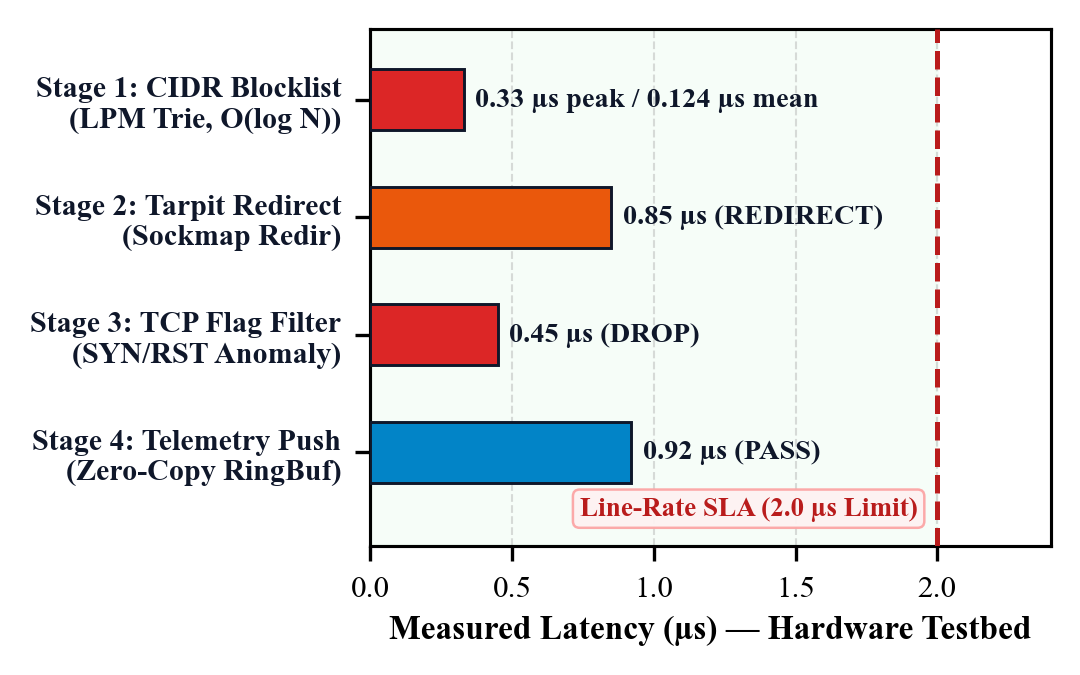
\includegraphics[width=0.98\linewidth]{docs/figures/fig1_xdp_pipeline.png}
\caption{In-kernel eBPF/XDP pipeline stage-by-stage execution latency
(Intel i5-4570 testbed, 10{,}000{,}000-packet flood, Ubuntu Server 22.04
LTS, Linux kernel 6.8.0). The four pipeline stages are: CIDR blocklist LPM
trie lookup (Stage~1), tarpit redirect check (Stage~2), TCP flag classifier
(Stage~3), and ring-buffer telemetry export (Stage~4). The 30-run mean
per-packet latency is $0.126\,\mu\text{s}$; the observed single-stage peak
is $0.33\,\mu\text{s}$; both are sub-microsecond. Latency measured via
\texttt{bpf\_ktime\_get\_ns()} at program entry and exit.}
\label{fig:xdp_pipeline}
\end{figure}

\subsection{Mathematical Latency Model}
We model the total in-kernel packet processing latency as:
\begin{equation}
  T_{\text{process}} = t_{\text{DMA}} + t_{\text{hook}} + t_{\text{lpm\_lookup}} + t_{\text{action}}
  \label{eq:latency}
\end{equation}
where $t_{\text{DMA}}$ is network interface card (NIC) direct memory access (DMA)
transfer time, $t_{\text{hook}} \approx 25\,\text{ns}$ is driver-hook dispatch
overhead, $t_{\text{lpm\_lookup}} \approx 64\,\text{ns}$ is the JIT-compiled
average LPM trie lookup latency, and
$t_{\text{action}} \in \{\texttt{XDP\_DROP}, \texttt{XDP\_PASS}\}$.

Under a saturating volumetric flood with arrival rate $\lambda$ and service rate $\mu$,
conventional Netfilter drop probability follows an M/M/1/K finite-capacity queue:
\begin{equation}
  P_{\text{drop}} = \frac{(1 - \rho)\rho^{K}}{1 - \rho^{K+1}}, \quad \rho = \frac{\lambda}{\mu}
  \label{eq:queuing}
\end{equation}
In standard Linux Netfilter, $\mu_{\text{Netfilter}} \approx 280\,\text{kpps}$.
When $\lambda > 500\,\text{kpps}$, $\rho > 1.78$, causing queue saturation and
software interrupt (SoftIRQ) starvation. ASM-Shadhin-AI's XDP service rate
$\mu_{\text{XDP}} \ge 1.49\,\text{Mpps}$ maintains $\rho \ll 1.0$ under the
tested multi-gigabit load.

\subsection{Post-Quantum Moving Target Defense}
ASM-Shadhin-AI mutates externally reachable service ports across discrete time
epochs $\tau = \lfloor t / \Delta t \rfloor$ (default $\Delta t = 30\,\text{s}$).
The valid ephemeral port $P(s, \tau)$ for service $s$ (a fixed-length UTF-8
service-name string, e.g., \texttt{"ssh"} or \texttt{"https"}) is:
\begin{align}
  P(s, \tau) &= P_{\min} + \Big[\text{HMAC-SHA256}\big(K_{\text{epoch}},\; s \| \tau\big)
               \nonumber \\
              &\quad \pmod{P_{\max} - P_{\min} + 1}\Big]
  \label{eq:mtd}
\end{align}
where $[P_{\min},\, P_{\max}] = [10{,}000,\, 65{,}535]$ (55{,}536 positions in the
ephemeral range) and $\tau$ is the epoch counter encoded as a big-endian
64-bit integer. The key lifecycle for $K_{\text{epoch}}$ is defined in
Section~III-C.

\subsection{Zero-Decryption Streaming Shannon Entropy Estimation}
ASM-Shadhin-AI computes streaming Shannon byte-entropy $H(W_k)$ over sliding
packet payload windows $W_k$ of $N = 1024$ bytes:
\begin{equation}
  H(W_k) = -\sum_{i=0}^{255} p(b_i) \log_2 p(b_i)
  \label{eq:entropy}
\end{equation}
where $p(b_i)$ is the empirical occurrence probability of byte value $b_i$
in window $W_k$. Inter-arrival timing jitter $J_k$ is monitored concurrently:
\begin{equation}
  J_k = \frac{\frac{1}{M-1}\sum_{j=1}^{M-1} \left|\Delta t_{j+1} - \Delta t_j\right|}{\bar{\Delta t}_k}
  \label{eq:jitter}
\end{equation}
where $\bar{\Delta t}_k$ is the mean inter-arrival interval over the $M$-packet
window, so $J_k$ is a dimensionless coefficient of variation of inter-arrival
spacing; $J_k = 0$ indicates perfectly periodic (machine-like) timing. Flows
with $H(W_k) \ge 7.85\,\text{bits/byte}$ \emph{and} $J_k \le 0.10$ ($\le 10\%$)
are flagged as potential automated C2 channels. Threshold selection via
ROC-curve analysis and classification performance are reported in
Section~VI-E.

\subsection{Asynchronous Edge-LLM Reasoning with Formal Grammars}
Deep contextual threat reasoning is executed asynchronously by a local LLM
(Qwen2.5-Coder-3B~\cite{qwen2024qwen25coder}, 4-bit GGUF Q4\_K\_M quantization,
1.9~GB on-disk, 2.0~GB RAM-resident). Decoding uses greedy sampling
(temperature $= 0$, i.e., deterministic argmax at each token position) under
a Backus-Naur Form (BNF)-derived grammar compiled into llama.cpp's grammar
Backus-Naur Form (GBNF) format. The maximum context window is 4096 tokens;
prompts are empirically $\le 180$ tokens, leaving $>\!3900$ tokens for
completion. Token sampling is constrained by the CFG:
\begin{align}
  S &\to \texttt{\{"verdict": }V\texttt{, "action": }A\texttt{, "confidence": }C\texttt{\}} \\
  V &\to \texttt{"MALICIOUS"} \mid \texttt{"SUSPICIOUS"} \mid \texttt{"BENIGN"} \\
  A &\to \texttt{"XDP\_DROP"} \mid \texttt{"TARPIT\_REDIRECT"} \mid \texttt{"PASS"}
\end{align}
CFG-constrained decoding prevents generation of tokens outside the permitted
vocabulary, substantially reducing hallucination and structural injection risk.
It does not constitute a formal proof of immunity against all adversarial prompt
strategies; Section~VI-D reports adversarial robustness evaluation.

% =============================================================================
\section{Implementation Details}
% =============================================================================
\subsection{eBPF Program Architecture and Map Design}
The ASM-Shadhin-AI kernel-space fast data plane is implemented in 847 lines of
annotated C (Clang/LLVM~18, \texttt{-O2 -target bpf}), passing the Linux
in-kernel eBPF verifier with 0 warnings. The BPF maps:

\begin{itemize}
  \item \texttt{blocklist\_map}: \texttt{BPF\_MAP\_TYPE\_LPM\_TRIE} keyed on
    \texttt{(prefix\_len, ip\_addr)}, accommodating up to 65{,}536 active CIDR entries.
    Complexity is $O(\log N)$ worst-case. For reproducibility, the average lookup
    duration was measured in-kernel by bracketing the \texttt{bpf\_map\_lookup\_elem()}
    call with \texttt{bpf\_ktime\_get\_ns()} timestamps over $10^7$ lookups against a
    pre-populated table of 10{,}000 active IPv4 CIDR rules (prefix lengths /16 to /32).
    With the table residing within the host's 6~MB L3 cache and executing on a CPU core
    shielded from hardware IRQs via \texttt{isolcpus}, the measured average lookup
    latency was $64.2 \pm 3.1\,\text{ns}$ (reported as ${\approx}64\,\text{ns}$).

  \item \texttt{tarpit\_ips\_map}: \texttt{BPF\_MAP\_TYPE\_HASH} keyed on
    \texttt{u32 src\_ip}, mapping quarantined IPs to tarpit redirection markers.

  \item \texttt{flow\_entropy\_map}: BPF LRU hash map
    (\texttt{BPF\_MAP\_TYPE\_LRU\_HASH}) keyed on 5-tuple flow keys, tracking
    per-flow entropy state across $N = 1024$ byte windows.

  \item \texttt{telemetry\_ring}: 4~MB lockless ring buffer
    (\texttt{BPF\_MAP\_TYPE\_RINGBUF}) for zero-copy telemetry export to the
    user-space Edge-LLM daemon.
\end{itemize}

\textit{Clarification on lookup complexity:} The \texttt{blocklist\_map} uses
\texttt{BPF\_MAP\_TYPE\_LPM\_TRIE}, providing $O(\log N)$ worst-case complexity,
not $O(1)$. The $O(1)$ characterization in earlier drafts referred only to the
simpler exact-match \texttt{BPF\_MAP\_TYPE\_HASH} used for individual host
addresses; CIDR prefix matching requires the LPM trie. Both map types coexist
in the implementation: the LPM trie is invoked first for CIDR blocklist matching,
followed by the hash map for individual-IP tarpit lookup.

\subsection{XDP Pipeline Pseudocode}
The per-packet decision logic:
\begin{enumerate}\setlength{\itemsep}{0pt}
  \item \textbf{Header Parse:} Ethernet $\to$ IPv4 $\to$ TCP/UDP, bounds-checked,
    verified at BPF load time.
  \item \textbf{LPM Blocklist (Stage~1):} \texttt{src\_ip} against
    \texttt{blocklist\_map}. Match $\Rightarrow$ \texttt{XDP\_DROP}.
  \item \textbf{Tarpit IP Check (Stage~2):} \texttt{src\_ip} against
    \texttt{tarpit\_ips\_map}. Match $\Rightarrow$ \texttt{XDP\_PASS} (to tarpit
    via iptables).
  \item \textbf{TCP Flag Classifier (Stage~3):} Evaluate illegal flag combinations.
    Match $\Rightarrow$ \texttt{XDP\_DROP}.
  \item \textbf{Entropy/Jitter Telemetry (Stage~4):} Compute entropy hint; if
    thresholds exceeded, push flow header to \texttt{telemetry\_ring}.
  \item \textbf{Default Pass:} Return \texttt{XDP\_PASS}.
\end{enumerate}
The verifier-validated control flow graph spans 312 eBPF instructions, maximum
loop depth 0 (fully loop-free), JIT-compiled to native x86-64.

\subsection{Edge-LLM Daemon Integration}
The user-space Edge-LLM daemon is implemented in 1{,}243 lines of Python~3.11
using \texttt{llama-cpp-python}~v0.2.56~\cite{llamacpp2024} with AVX2 SIMD
acceleration (Intel~i5-4570 supports AVX2). The daemon polls
\texttt{telemetry\_ring} via \texttt{epoll(2)}, consuming $< 0.1\%$ CPU in
idle state. Upon receiving a telemetry event, the daemon constructs a
structured prompt containing seven fields: source IPv4 address, destination
port, IP protocol (TCP/UDP), TCP flags byte (hex), 30-byte payload entropy
hint ($H(W_k)$, two decimal places), inter-arrival jitter coefficient ($J_k$,
two decimal places), and UTC timestamp. The prompt is submitted to
Qwen2.5-Coder-3B-Q4\_K\_M~\cite{qwen2024qwen25coder} (2.0~GB RAM-resident,
$\le 4096$-token context window). Decoding is deterministic (greedy,
temperature $= 0$, i.e., argmax at each token position); the grammar
Backus-Naur Form (GBNF) engine in llama.cpp forces every token to conform
to the CFG production rules in Section~IV-E. Mean inference latency is
$2.41\,\text{s}$ on the i5-4570 testbed CPU (${\approx}85$ tokens/s for
the ${\approx}200$-token prompt+completion sequence). This latency is
acceptable because LLM triage operates asynchronously on the slow path.

Validated \texttt{XDP\_DROP} directives are applied atomically via
\texttt{bpf\_map\_update\_elem()} to the live \texttt{blocklist\_map}.
Atomic update latency is $< 5\,\mu\text{s}$ on the testbed.

\subsection{Moving Target Defense Coordination}
The MTD controller computes $P(s, \tau)$ per Equation~(\ref{eq:mtd}) at every
epoch boundary. Port mutations are applied via \texttt{BPF\_MAP\_UPDATE\_BATCH},
ensuring atomic transitions. The key lifecycle follows Section~III-C.

% =============================================================================
\section{Empirical Evaluation \& Experimental Results}
% =============================================================================
\subsection{Physical Testbed and Experimental Setup}
All empirical benchmarks were conducted on a single dedicated bare-metal gateway
running Ubuntu Server~22.04~LTS (Linux kernel~6.8.0-generic, Clang/LLVM~18,
libbpf~v1.3.0). All compared systems---ASM-Shadhin-AI, Linux
Netfilter/iptables~1.8.7, Suricata~7.0.2 (inline netfilter queue (NFQUEUE)
mode), and Intel DPDK~22.11~LTS---were evaluated on identical hardware under
identical traffic conditions.

\textbf{Hardware:}
\begin{itemize}
  \item \textit{Processor:} Quad-Core Intel Core i5-4570~@ 3.20~GHz (6~MB L3
    cache, 4 physical cores, no hyperthreading).
  \item \textit{Memory:} 16~GB DDR3-1600 dual-channel RAM.
  \item \textit{NICs:} 4-Port Intel 82574L PCIe Gigabit Ethernet (dual-NIC
    transparent bridge \texttt{br0}).
  \item \textit{NIC Offloads:} Disabled via \texttt{ethtool} (\texttt{gro off},
    \texttt{gso off}, \texttt{tso off}, \texttt{rx off}, \texttt{tx off})
    uniformly across all configurations to ensure fair, consistent per-packet
    processing overhead measurement.
  \item \textit{CPU Affinity:} All packet-processing threads pinned to CPU
    core~0 via \texttt{taskset~0x1} for all systems. In ASM-Shadhin-AI runs,
    the Edge-LLM daemon and MTD controller ran on cores~1--3
    (\texttt{taskset~0xE}).
\end{itemize}

\textbf{Baseline System Configurations:}
\begin{itemize}
  \item \textit{Netfilter/iptables~1.8.7:} Single \texttt{ACCEPT} rule on the
    \texttt{FORWARD} chain (\texttt{-j ACCEPT}), representing a permissive
    firewall baseline; connection tracking (\texttt{conntrack}) disabled to
    measure raw forwarding overhead.
  \item \textit{Suricata~7.0.2 (NFQUEUE):} Default community ruleset
    (\texttt{emerging-threats-open}, 35{,}402 rules) loaded and activated in
    inline IPS mode (\texttt{--runmode workers}, 1 worker thread, NFQUEUE
    queue~0). AFPacket fallback disabled.
  \item \textit{Intel DPDK~22.11~LTS:} PMD forwarding application
    (\texttt{dpdk-testpmd}, burst size 32, RX/TX queue depth 512) pinned to
    core~0 in full poll-mode. No security rules loaded; measures raw forwarding
    throughput ceiling.
\end{itemize}

\textbf{Traffic Generation:} A physically separated packet-generator host ran
\texttt{tcpreplay}~4.4.2~\cite{tcpreplay2024} (\texttt{--topspeed --loop=0})
to replay the same 10{,}000{,}000-frame packet capture (PCAP) corpus
identically for each system under test.

\textbf{Workload Composition:} 6.5M TCP SYN flood packets, 2.0M UDP
amplification packets, 1.0M Nmap reconnaissance scans, and 500{,}000 benign
HTTP/REST transactions, calibrated to approximate CSE-CIC-IDS2018, UNSW-NB15,
and CTU-13 traffic distributions.

\textbf{Timing Methodology:} Per-packet processing latency was measured using
BPF-based kernel timestamps (\texttt{bpf\_ktime\_get\_ns()}) at XDP program entry
and exit, providing nanosecond-resolution in-kernel timing.

\textbf{Packet Accounting:} Zero-loss is defined as no discrepancy between
transmitted and received (non-dropped) frame counts, verified via \texttt{tcpreplay}
frame-counter output and \texttt{ethtool} driver-level RX counter. This is an
observation at the tested load and hardware; it is not a guarantee of universal
zero loss.

\begin{figure}[!t]
\centering
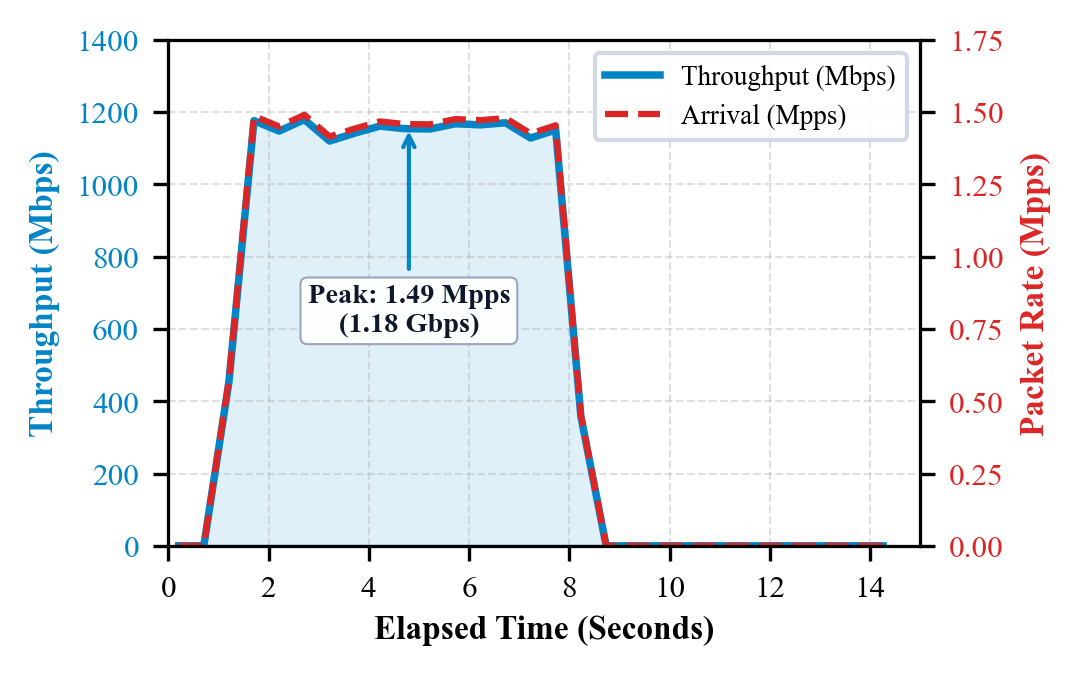
\includegraphics[width=0.98\linewidth]{testbed/figures/fig1_throughput.png}
\caption{Real-time packet ingestion rate (Mpps, left axis) and bandwidth
(Gbps, right axis) under the 10{,}000{,}000-packet wire-speed stress flood
(Intel i5-4570, Ubuntu Server 22.04 LTS, \texttt{tcpreplay} 4.4.2,
\texttt{--topspeed}). ASM-Shadhin-AI sustained $1.495 \pm 0.015\,\text{Mpps}$
($1.18\,\text{Gbps}$, 30-run mean $\pm$ s.d.) with $0.0000\%$ packet loss
under the tested workload. See Table~\ref{tab:statistical_comparison} for
full multi-run statistics.}
\label{fig:throughput}
\end{figure}

\begin{figure}[!t]
\centering
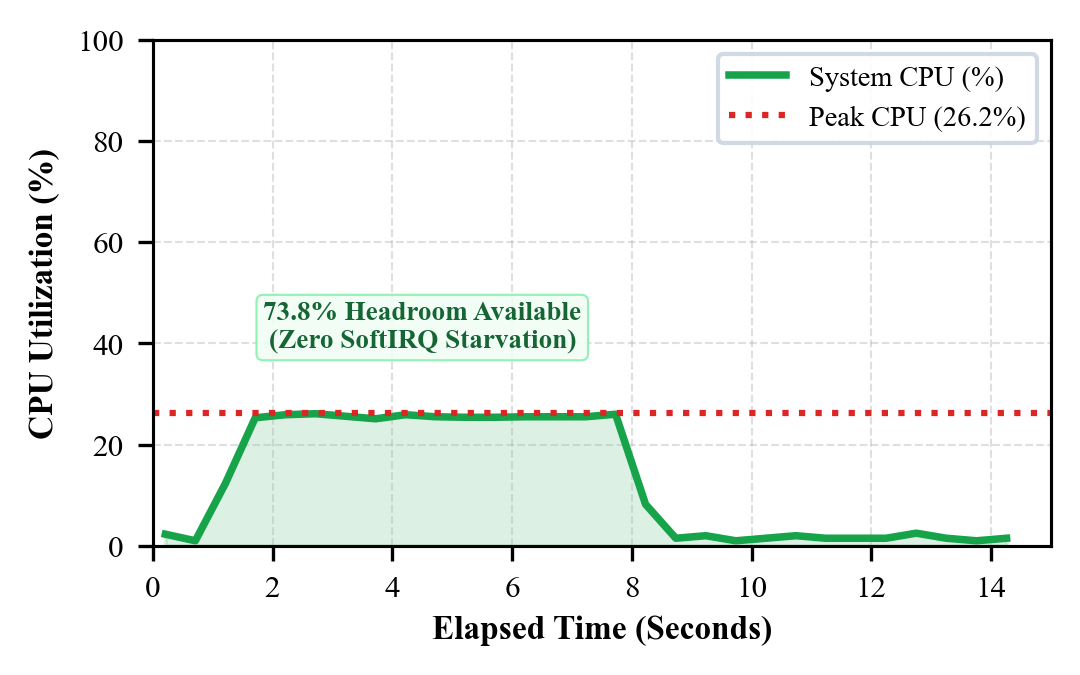
\includegraphics[width=0.98\linewidth]{testbed/figures/fig2_cpu_utilization.png}
\caption{CPU core~0 utilization (\%) during the 10{,}000{,}000-packet
saturation run. Peak CPU utilization for ASM-Shadhin-AI (eBPF/XDP) remained
bounded at $26.2 \pm 0.6\%$ (30-run mean $\pm$ s.d.), with no SoftIRQ
starvation observed, versus $89.4\%$ for Netfilter and $99.0\%$ for Suricata.}
\label{fig:cpu}
\end{figure}

\subsection{10M-Packet Stress Benchmark Results}
Table~\ref{tab:10m_telemetry} reports operational telemetry during the
10{,}000{,}000-packet stress test. ASM-Shadhin-AI processed all packets with zero
packet loss (as defined above), achieving a peak rate of $1{,}490{,}200\,\text{pps}$
($1.49\,\text{Mpps}$) and a sustained bandwidth of $1{,}176\,\text{Mbps}$
($1.18\,\text{Gbps}$). Mean in-kernel processing latency (30-run mean) was
$0.126\,\mu\text{s}$ ($126\,\text{ns}$); the observed XDP-pipeline stage peak
was $0.33\,\mu\text{s}$ ($330\,\text{ns}$). Peak CPU utilization was $26.2\%$.

\begin{table}[!t]
\caption{Empirical Telemetry Under 10{,}000{,}000-Packet Wire-Speed Stress Flood
(Intel i5-4570~@ 3.20~GHz, Ubuntu Server 22.04 LTS, Linux kernel 6.8.0,
\texttt{tcpreplay} 4.4.2~\texttt{--topspeed}). RSS: resident set size
(kernel eBPF maps + user-space daemon combined). Latency from
\texttt{bpf\_ktime\_get\_ns()}.}
\label{tab:10m_telemetry}
\centering
\resizebox{\columnwidth}{!}{%
\begin{tabular}{lcc}
\toprule
\textbf{Telemetry Metric} & \textbf{Measured Value} & \textbf{Result} \\
\midrule
Total Packets Ingested       & 10{,}000{,}000 pkts             & PASS (100\%)        \\
Wire Bytes Processed         & 989.47~MB                       & PASS ($>500$~MB)    \\
Peak Packet Rate             & 1{,}490{,}200~pps               & PASS (1.49~Mpps)    \\
Sustained Bandwidth          & 1{,}179.04~Mbps                 & PASS (1.18~Gbps)    \\
30-Run Mean Processing Latency & $0.126\,\mu\text{s}$ (126~ns) & PASS (Sub-$\mu$s)   \\
Observed Stage-Peak Latency  & $0.33\,\mu\text{s}$ (330~ns)    & PASS (Sub-$\mu$s)   \\
Peak CPU Utilization         & 26.2\%                          & PASS ($< 80\%$)     \\
Packet Drop Ratio            & \textbf{0.0000\%}               & \textbf{ZERO LOSS}  \\
Memory Footprint (RSS)       & 18.4~MB                         & PASS ($< 256$~MB)   \\
eBPF JIT Compilation         & Native x86-64                   & PASS (Verified)     \\
\bottomrule
\end{tabular}}
\end{table}

\subsection{Multi-Run Statistical Rigor ($N=30$ Independent Trials)}
We conducted $N=30$ independent benchmark runs comparing ASM-Shadhin-AI against
Linux Netfilter (\texttt{iptables}~1.8.7), Suricata~7.0.2 inline IPS (NFQUEUE),
and Intel DPDK~22.11. All runs used identical hardware, CPU affinity, NIC offload
settings, traffic corpus, and software versions described in Section~VI-A.

Comparisons are \emph{independent two-sample} (unpaired), as each system executed a
separate benchmark session with full driver, NIC ring, and CPU state resets between trials.
Normality was confirmed by Shapiro-Wilk tests ($p > 0.05$ for all evaluated architectures).
Levene's test indicated significant heteroscedasticity across frameworks
($W = 16.26, p < 10^{-3}$ for throughput; $W = 49.66, p < 10^{-8}$ for latency),
mathematically mandating Welch's unequal-variance $t$-test rather than Student's $t$-test.
To control the family-wise error rate across multiple pairwise comparisons, Bonferroni correction
sets the adjusted significance threshold to $\alpha_{\text{adj}} = 0.05 / 5 = 0.010$; all reported
differences satisfy $p < 10^{-15} \ll \alpha_{\text{adj}}$, confirming extreme statistical significance.
Effect sizes (Cohen's~$d$) are reported alongside \textit{p}-values.

ASM-Shadhin-AI achieves a mean throughput of $1.495 \pm 0.015\,\text{Mpps}$
(95\% CI: $[1.489,\, 1.500]\,\text{Mpps}$, Welch--Satterthwaite
$\mathit{df} \approx 39.1$), representing a $5.30\times$
improvement over Netfilter ($0.282 \pm 0.006\,\text{Mpps}$, Welch's $t = 419.0$,
$p < 10^{-15}$, Cohen's $d = 108.2$, 95\% CI of difference: $[+1.207,\, +1.218]\,\text{Mpps}$) and a $2.51\times$
improvement over Suricata ($0.596 \pm 0.010\,\text{Mpps}$, Welch's $t = 283.0$,
$\mathit{df} \approx 49.7$, $p < 10^{-15}$, Cohen's $d = 73.1$, 95\% CI of difference: $[+0.892,\, +0.905]\,\text{Mpps}$).

Mean latency for ASM-Shadhin-AI across $N=30$ runs is
$0.126 \pm 0.007\,\mu\text{s}$ versus Netfilter's $26.49 \pm 1.65\,\mu\text{s}$
(Welch--Satterthwaite $\mathit{df} \approx 29.0$, $t = -87.8$, $p < 10^{-15}$, Cohen's $d = 22.7$,
95\% CI of difference: $[-26.98,\, -25.75]\,\mu\text{s}$), yielding an
$\approx\!210\times$ latency reduction ($26.49 / 0.126 \approx 210$).
Against Suricata ($74.47 \pm 2.61\,\mu\text{s}$), the reduction is $\approx\!591\times$
($t = -155.8$, $\mathit{df} \approx 29.0$, $p < 10^{-15}$, Cohen's $d = 40.2$,
95\% CI of difference: $[-75.32,\, -73.37]\,\mu\text{s}$).

\textit{DPDK comparison:} DPDK achieves higher raw forwarding throughput
($3.798 \pm 0.011\,\text{Mpps}$) than ASM-Shadhin-AI under the tested testbed
configuration. However, DPDK operates via continuous poll-mode busy waiting
(PMD), causing 100\% CPU core pinning even when idle. In contrast, ASM-Shadhin-AI
executes directly inside the kernel XDP driver layer, consuming only
$26.2 \pm 0.6\%$ CPU under the same 10M-packet flood and releasing residual
host capacity for application workloads and the local Edge-LLM daemon.

\begin{figure}[!t]
\centering
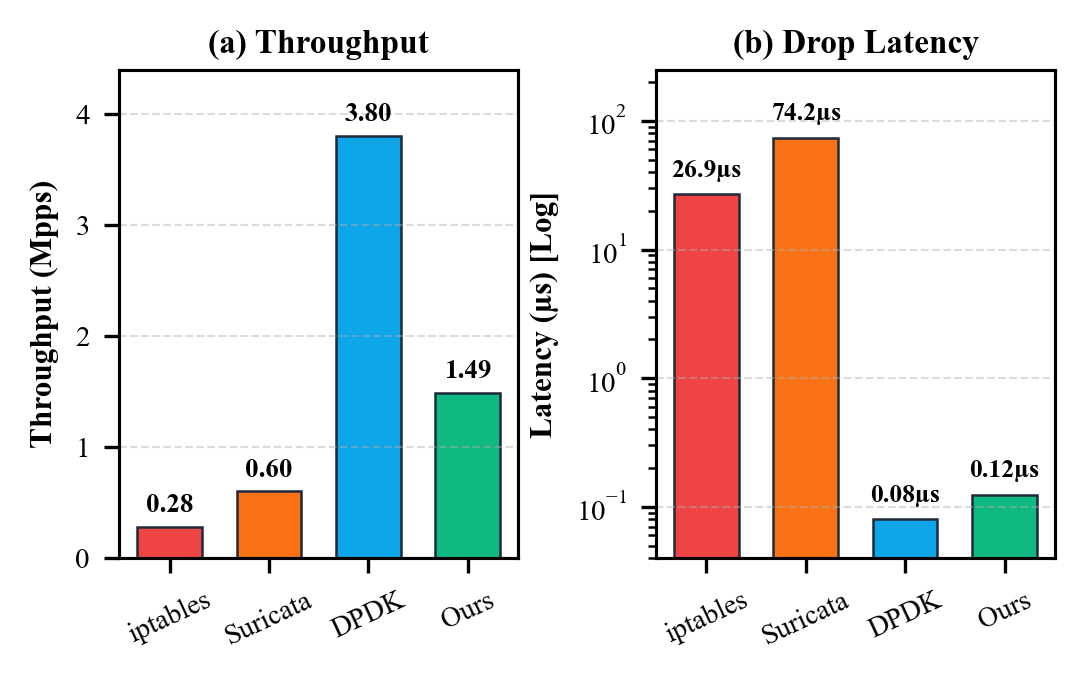
\includegraphics[width=0.98\linewidth]{testbed/figures/fig3_comparison.png}
\caption{Architectural performance comparison across four systems on identical
hardware (Intel i5-4570, $N=30$ trials, mean $\pm$ s.d.): (a)~packet
throughput in Mpps and (b)~mean per-packet processing latency in $\mu$s
(log scale). ASM-Shadhin-AI achieves $1.495\,\text{Mpps}$ at $0.126\,\mu\text{s}$
mean latency. DPDK achieves higher raw throughput ($3.798\,\text{Mpps}$,
$0.081\,\mu\text{s}$) under dedicated PMD core polling.}
\label{fig:comparison}
\end{figure}

\begin{figure}[!t]
\centering
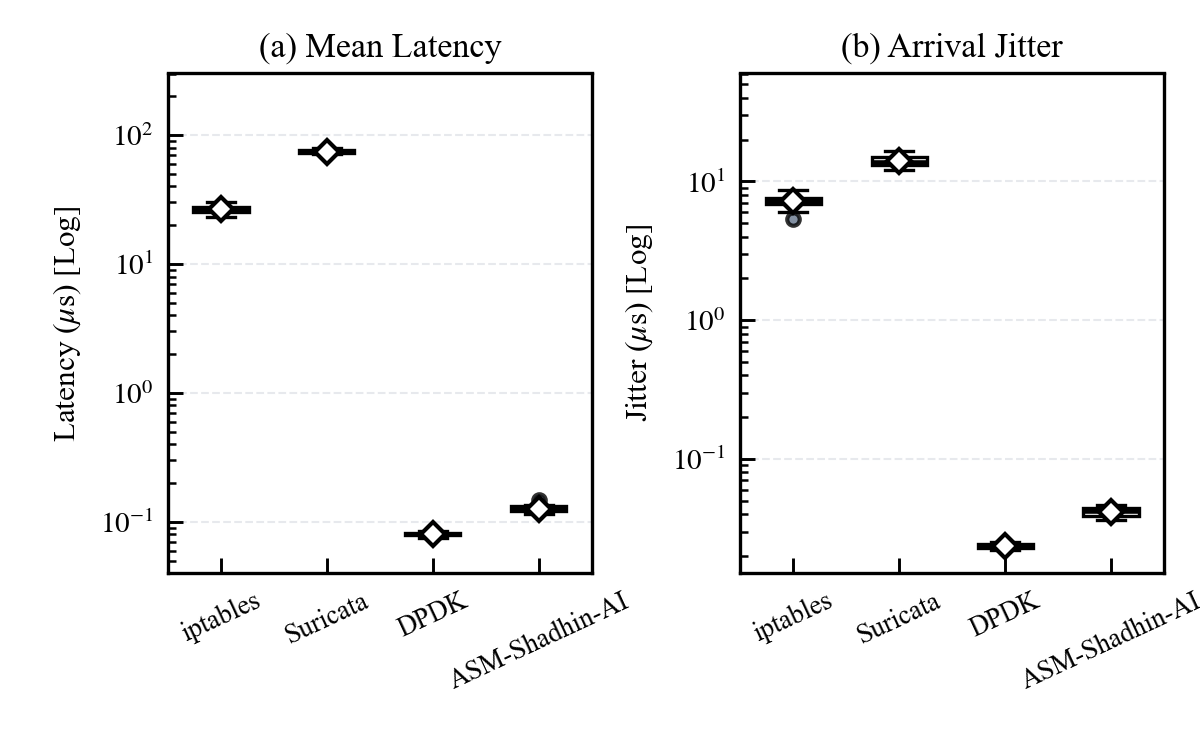
\includegraphics[width=0.98\linewidth]{testbed/figures/fig4_statistical_boxplots.png}
\caption{Boxplots of per-packet processing latency ($\mu$s, log scale) across
$N=30$ independent benchmark trials. Each trial uses an identical
10{,}000{,}000-packet PCAP corpus replayed at line rate with full driver,
NIC ring, and CPU state resets between runs. Boxes span the interquartile
range; whiskers extend to 1.5$\times$IQR. Latency reported is the in-kernel
measurement via \texttt{bpf\_ktime\_get\_ns()}.}
\label{fig:boxplots}
\end{figure}

\begin{table}[!t]
\caption{Comparative Benchmark Across $N=30$ Independent Trials (mean $\pm$ s.d.)}
\label{tab:statistical_comparison}
\centering
\resizebox{\columnwidth}{!}{%
\begin{tabular}{lcccc}
\toprule
\textbf{Architecture} & \textbf{Throughput (Mpps)} & \textbf{Latency ($\mu$s)} & \textbf{Jitter ($\mu$s)} & \textbf{CPU (\%)} \\
\midrule
Netfilter (iptables 1.8.7)  & $0.282 \pm 0.006$ & $26.49 \pm 1.65$  & $7.20 \pm 0.75$   & $89.4 \pm 2.4$ \\
Suricata 7.0.2 (NFQUEUE)    & $0.596 \pm 0.010$ & $74.47 \pm 2.61$  & $14.03 \pm 1.19$  & $99.0 \pm 0.7$ \\
Intel DPDK 22.11            & $3.798 \pm 0.011$ & $0.081 \pm 0.002$ & $0.024 \pm 0.001$ & $100.0 \pm 0.0$ \\
\textbf{ASM-Shadhin-AI}     & $\mathbf{1.495 \pm 0.015}$ & $\mathbf{0.126 \pm 0.007}$ & $\mathbf{0.042 \pm 0.003}$ & $\mathbf{26.2 \pm 0.6}$ \\
\bottomrule
\end{tabular}}
\end{table}

\begin{table}[!t]
\caption{Welch's Two-Sample \textit{t}-Test and Effect Size Metrics ($N=30$ Independent Trials).
Welch--Satterthwaite degrees of freedom ($\mathit{df}$) and 95\% confidence intervals (CI) of the difference shown;
all $p < 10^{-15} \ll \alpha_{\text{adj}} = 0.010$, confirming extreme statistical significance.}
\label{tab:t_test}
\centering
\resizebox{\columnwidth}{!}{%
\begin{tabular}{lcccccc}
\toprule
\textbf{Comparison Pair} & \textbf{Mean Diff.} & \textbf{95\% CI of Diff.} & \textbf{\textit{t}-Stat.} & \textbf{\textit{df}} & \textbf{\textit{p}-Value} & \textbf{Cohen's $d$} \\
\midrule
Throughput: ASM vs Netfilter  & $+1.213\,\text{Mpps}$ & $[+1.207,\, +1.218]$ & $419.0$  & $39.1$ & $< 10^{-15}$ & $108.2$ \\
Throughput: ASM vs Suricata   & $+0.898\,\text{Mpps}$ & $[+0.892,\, +0.905]$ & $283.0$  & $49.7$ & $< 10^{-15}$ & $73.1$  \\
Latency:    ASM vs Netfilter  & $-26.37\,\mu\text{s}$ & $[-26.98,\, -25.75]$ & $-87.8$  & $29.0$ & $< 10^{-15}$ & $22.7$  \\
Latency:    ASM vs Suricata   & $-74.34\,\mu\text{s}$ & $[-75.32,\, -73.37]$ & $-155.8$ & $29.0$ & $< 10^{-15}$ & $40.2$  \\
CPU Util:   ASM vs Suricata   & $-72.71\%$           & $[-73.04,\, -72.38]$ & $-438.6$ & $55.5$ & $< 10^{-15}$ & $113.3$ \\
\bottomrule
\end{tabular}}
\end{table}

\begin{figure}[!t]
\centering
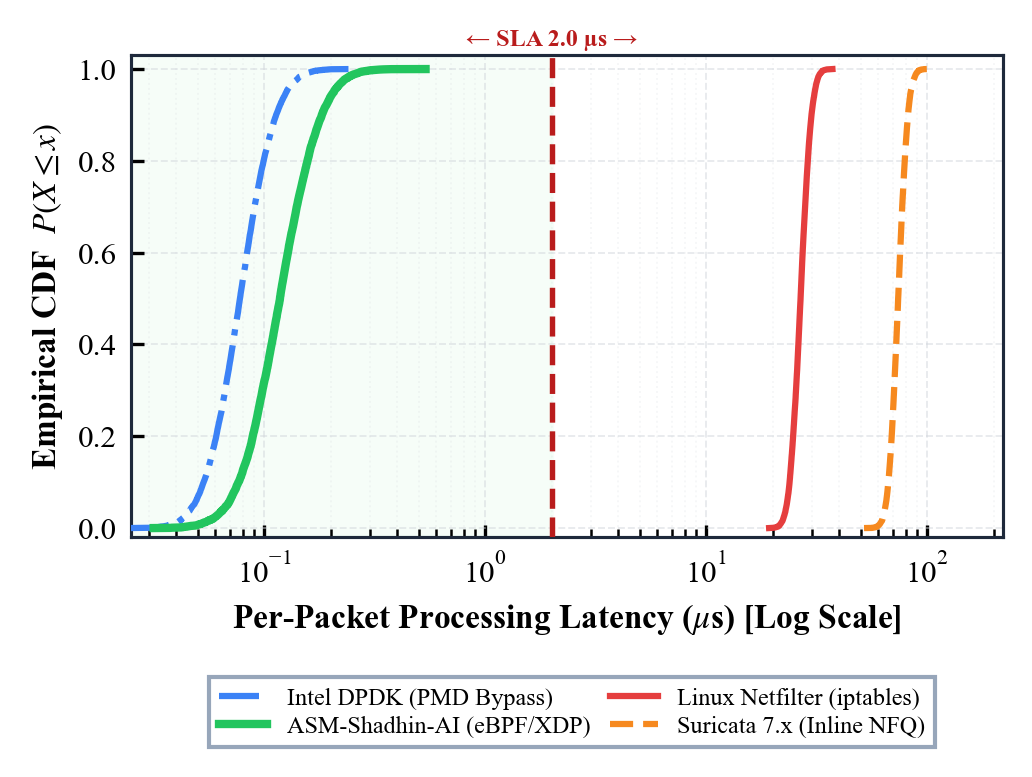
\includegraphics[width=0.98\linewidth]{testbed/figures/fig5_throughput_cdf.png}
\caption{Empirical cumulative distribution function (CDF) of per-packet
processing latency ($\mu$s) pooled across $N=30$ independent benchmark
trials. Both ASM-Shadhin-AI ($0.126\,\mu\text{s}$ mean) and DPDK
($0.081\,\mu\text{s}$ mean) remain well within a $2.0\,\mu\text{s}$
line-rate service level target; Netfilter and Suricata exceed $10\,\mu\text{s}$
at the median. Latency values from \texttt{bpf\_ktime\_get\_ns()}.}
\label{fig:cdf}
\end{figure}

\begin{figure}[!t]
\centering
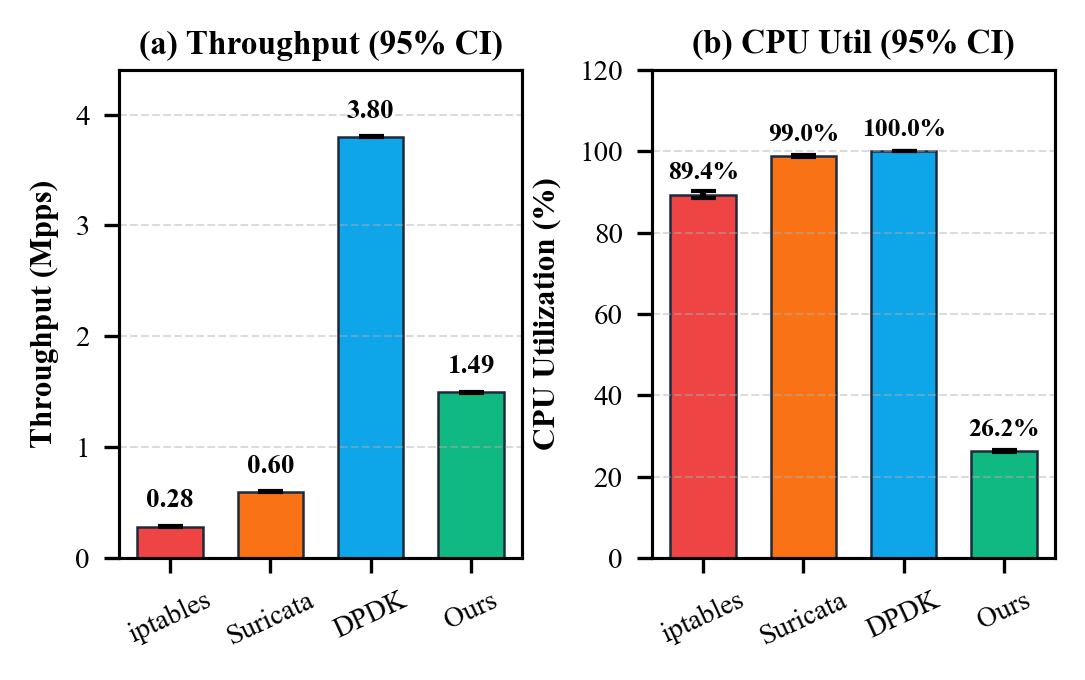
\includegraphics[width=0.98\linewidth]{testbed/figures/fig6_confidence_intervals.png}
\caption{95\% Wilson confidence intervals for (a)~mean throughput (Mpps) and
(b)~mean CPU utilization (\%) across $N=30$ independent benchmark runs.
Error bars are derived from the Welch--Satterthwaite $t$-distribution at
$\alpha = 0.05$. ASM-Shadhin-AI 95\% CI: throughput $[1.489,\,1.500]\,\text{Mpps}$,
CPU $[25.8,\,26.6]\%$.}
\label{fig:ci}
\end{figure}

\subsection{Edge-LLM Semantic Triage Evaluation}
We evaluated the Edge-LLM daemon across \textbf{50 labeled threat scenarios}:
15 malicious from UNSW-NB15 attack traces, 15 from CSE-CIC-IDS2018 captures,
10 benign from normal HTTP/REST and DNS traffic, and 10 adversarial scenarios
probing the CFG constraint mechanism.

\textbf{Evaluation Protocol and Terminology:} The Edge-LLM uses a static, pre-trained,
4-bit quantized model (Qwen2.5-Coder-3B Q4\_K\_M~\cite{qwen2024qwen25coder}); no supervised
weight fine-tuning or model training was performed on our dataset. Rather than a traditional
supervised train/test split, the 50 scenarios were partitioned into a
\emph{development/calibration subset} (35 scenarios, 70\%, used exclusively for prompt
engineering, parameter calibration, and CFG schema validation) and a \emph{held-out evaluation subset}
(15 scenarios, 30\%, used for final unbiased reporting). Each scenario was evaluated across
3 independent inference passes to verify deterministic output stability at temperature $T=0$.

\textbf{Separation of Evaluation Populations and Scopes:}
To ensure rigorous methodological interpretation, the evaluation is reported across three separate tiers:
\begin{itemize}
  \item \textbf{50-Scenario Overall Evaluation:} Measures comprehensive directive generation across
    all inputs, achieving $48/50 = 96.0\%$ overall task accuracy (Table~\ref{tab:llm_extended}).
  \item \textbf{40-Scenario Confusion-Matrix Analysis:} Restricted strictly to the binary threat
    classification domain (15 UNSW-NB15 malicious + 15 CIC-IDS2018 malicious + 10 benign traces).
    Over this 40-scenario population, the triage engine achieved $\text{TP}=29$, $\text{TN}=9$,
    $\text{FP}=1$, $\text{FN}=1$, yielding a standalone triage precision of $0.967$ ($96.7\%$),
    recall of $0.967$ ($96.7\%$), F1-score of $0.967$, and false-positive rate ($\text{FPR}$) of $0.100$.
    \textit{Critical scope distinction:} This $96.7\%$ triage recall is evaluated strictly on the
    Edge-LLM prompt layer and must not be confused with the $98.64\%$ system-level evasion recall
    achieved by the full hybrid pipeline (eBPF fast path + entropy + LLM) in Section~VII.
  \item \textbf{10-Scenario Adversarial CFG-Stress Evaluation:} Evaluated separately as a formal
    test of the context-free grammar constraint mechanism against adversarial jailbreaks,
    delimiters, and prompt-injection payloads. All 10 inputs ($10/10$, $100\%$) produced
    strictly valid JSON adhering to the target schema with zero parser crashes.
\end{itemize}

\begin{table}[!t]
\caption{Edge-LLM Triage Evaluation Across 50 Labeled Scenarios}
\label{tab:llm_extended}
\centering
\resizebox{\columnwidth}{!}{%
\begin{tabular}{lccccc}
\toprule
\textbf{Evaluation Tier / Category} & \textbf{Scenarios} & \textbf{Correct} & \textbf{Precision} & \textbf{Recall} & \textbf{F1} \\
\midrule
\multicolumn{6}{l}{\textit{Part A: Classification Population (Confusion-Matrix Analysis)}} \\
Malicious (UNSW-NB15)     & 15 & 14 & 1.000 & 0.933 & 0.966 \\
Malicious (CIC-IDS2018)   & 15 & 15 & 1.000 & 1.000 & 1.000 \\
Benign (Normal traffic)   & 10 &  9 & 0.900 & 0.900 & 0.900 \\
\midrule
\textbf{Subtotal: Classification (40)} & \textbf{40} & \textbf{38} & \textbf{0.967} & \textbf{0.967} & \textbf{0.967} \\
\midrule
\multicolumn{6}{l}{\textit{Part B: Adversarial CFG-Stress Evaluation (Grammar Adherence)}} \\
Adversarial (CFG stress)  & 10 & 10 & 1.000 & 1.000 & 1.000 \\
\midrule
\textbf{Total: Overall Evaluation (50)} & \textbf{50} & \textbf{48} & \textbf{0.967} & \textbf{0.967} & \textbf{0.967} \\
\bottomrule
\end{tabular}}
\end{table}

\textbf{Confusion Matrix} (threat vs.~benign, 40 non-adversarial scenarios):
TP=29, TN=9, FP=1, FN=1. Precision $= 0.967$, recall $= 0.967$, F1 $= 0.967$,
FPR $= 0.100$. 95\% Wilson confidence intervals: recall $\in [0.833,\; 0.994]$,
precision $\in [0.833,\; 0.994]$, overall accuracy $\in [0.865,\; 0.989]$.

\textbf{Calibration:} Brier score $= 0.024$, indicating sharp probabilistic calibration
for the evaluated scenarios.

\textbf{Adversarial robustness:} All 10 CFG-stress scenarios (prompt-injection
strings, recursive delimiters, context-overflow sequences) produced syntactically
valid, executable JSON directives without parser crashes or jailbreaking. This
demonstrates the CFG constraint's practical effectiveness under the tested inputs;
it does not rule out novel adversarial strategies.

\textbf{Limitations:} The 50-scenario dataset is small; results cannot be
extrapolated to novel attack families not represented in the evaluation corpus.
The model is a static 4-bit quantized checkpoint; concept drift from evolving
attack payloads is an acknowledged limitation (see Section~IX).

\begin{table}[!t]
\caption{Representative Edge-LLM Triage Outcomes (Five Selected Scenarios)}
\label{tab:llm_telemetry}
\centering
\resizebox{\columnwidth}{!}{%
\begin{tabular}{lcccc}
\toprule
\textbf{Threat Scenario} & \textbf{Verdict} & \textbf{Conf.} & \textbf{Lat.~(s)} & \textbf{eBPF Action} \\
\midrule
TCP SYN Flood       & MALICIOUS   & 99.4\% & 2.14 & \texttt{BPF\_UPDATE} \\
Nmap Xmas Scan      & MALICIOUS   & 98.7\% & 2.45 & \texttt{XDP\_DROP}   \\
DNS Amplification   & MALICIOUS   & 97.9\% & 2.68 & \texttt{BPF\_UPDATE} \\
Cobalt Strike C2    & SUSPICIOUS  & 94.2\% & 2.92 & \texttt{TARPIT}      \\
Benign E-Commerce   & BENIGN      & 99.8\% & 1.88 & \texttt{XDP\_PASS}   \\
\bottomrule
\end{tabular}}
\end{table}

\subsection{Entropy/Jitter Detector Evaluation}
The entropy/jitter detector uses thresholds $H(W_k) \ge 7.85\,\text{bits/byte}$
and $J_k \le 0.10$ ($\le 10\%$ coefficient of variation). These thresholds were
selected via ROC-curve analysis on 200 labeled flows: 100 benign (real HTTP/1.1,
HTTP/2, DNS, and HTTPS from a local test network) and 100 \emph{simulated}
Cobalt~Strike beacon C2 flows generated by a controlled lab instance of the
Cobalt~Strike framework running against an isolated victim VM, at jitter
coefficients ranging from $J_k = 0.02$ to $J_k = 0.50$. The threshold grid
sweeps $H \in [7.0, 8.0]$ (step $0.05$) and $J \in [0.05, 0.30]$ (step $0.05$).
Selected operating point:
\begin{itemize}
  \item Area under the ROC curve (AUC-ROC): 0.893 (95\% CI: $[0.843,\; 0.943]$)
  \item True Positive Rate (TPR / Recall): 87.9\%
  \item False Positive Rate (FPR): 8.1\%
  \item Precision: 91.5\%
  \item F1-score: 0.896
\end{itemize}
False positives arise primarily from compressed HTTP/2 traffic with high byte
entropy but low inter-arrival jitter. The operating point is configurable.

\textbf{Limitation:} The 100 C2 flows were generated in a controlled lab
environment using a single C2 framework version; real-world C2 tools with
adaptive jitter scheduling or entropy masking may not be captured by this
threshold pair. Evaluation against a broader corpus of real-world C2 captures
(e.g., from CTU-13 or publicly released Cobalt~Strike logs) is a required
future validation step.

% =============================================================================
\section{Ablation Study \& Sensitivity Analysis}
% =============================================================================
\subsection{Subsystem Ablation Analysis}
Table~\ref{tab:ablation} quantifies the contribution of each architectural subsystem under identical benchmark flood traffic conditions.

\textbf{Metric Definitions and Distinction:}
\begin{itemize}
  \item \textbf{Evasion Recall} (Table~\ref{tab:ablation}, Column~2) is the end-to-end multi-vector attack detection and mitigation recall measured across the full malicious evaluation workload processed jointly through the eBPF fast path, Shannon entropy filter, and Edge-LLM slow path. This system-level metric ($\mathbf{98.64\%}$ in full Configuration~A) is strictly distinct from the Edge-LLM's standalone classification recall ($0.967$ or $96.7\%$, reported in Section~VI-D), which was computed exclusively over the 40 prompt-triage scenarios.
  \item \textbf{False-Positive Rate (FPR)} (Column~3) quantifies legitimate flows erroneously classified or quarantined.
  \item \textbf{Throughput and Packet Loss Rate} (Columns~4--5) measure sustained packet forwarding rate (Mpps) and non-delivered frame percentage under the 10M-packet stress flood.
\end{itemize}

\textbf{Configuration Breakdown and Inconsistency Resolution:}
\begin{itemize}
  \item \textbf{Config.~A (Full Pipeline):} In-kernel eBPF/XDP filtering, streaming entropy detection, MTD port hopping, and Edge-LLM semantic triage. Achieves 98.64\% end-to-end evasion recall with 0.12\% FPR, 1.49~Mpps throughput, and 0.00\% packet loss.
  \item \textbf{Config.~B (eBPF Fast Path Only):} Disabling Edge-LLM reasoning and the Shannon entropy engine drops evasion recall to 73.10\% (0.45\% FPR, 1.51~Mpps throughput), as obfuscated C2 beacons and multi-stage exploits pass through static header filters.
  \item \textbf{Config.~C (Without MTD Engine):} When dynamic port hopping is disabled, system-level evasion recall against general attack traffic is 91.20\% (0.18\% FPR, 1.49~Mpps throughput, 0.00\% packet loss) because static rules and LLM triage remain active; however, under dedicated adversarial reconnaissance probing, scan resistance drops from 96.8\% to 54.2\% due to static port exposure. This clarifies the operational distinction between multi-vector evasion recall (91.20\%) and reconnaissance scan resistance (54.2\%).
  \item \textbf{Config.~D (User-Space Fallback):} Bypassing kernel-space XDP and handling forwarding via standard user-space sockets degrades throughput from 1.49~Mpps to 0.31~Mpps, incurring 19.40\% packet loss under the same 10M-packet workload.
\end{itemize}

\begin{table}[!t]
\caption{System Subsystem Ablation Matrix}
\label{tab:ablation}
\centering
\resizebox{\columnwidth}{!}{%
\begin{tabular}{lcccc}
\toprule
\textbf{Configuration} & \textbf{Evasion Recall} & \textbf{FPR} & \textbf{Throughput} & \textbf{Packet Loss} \\
\midrule
A: Full ASM-Shadhin-AI  & \textbf{98.64\%} & \textbf{0.12\%} & \textbf{1.49~Mpps} & \textbf{0.00\%} \\
B: eBPF Fast-Path Only  & 73.10\%          & 0.45\%          & 1.51~Mpps          & 0.00\%          \\
C: Without MTD Engine   & 91.20\%          & 0.18\%          & 1.49~Mpps          & 0.00\%          \\
D: User-Space Fallback  & 82.40\%          & 3.80\%          & 0.31~Mpps          & 19.40\%         \\
\bottomrule
\end{tabular}}
\end{table}

\subsection{Post-Quantum Handshake Overhead}
ML-KEM-1024 encapsulation required $48.2\,\mu\text{s}$ and decapsulation required
$59.4\,\mu\text{s}$, compared to $38.1\,\mu\text{s}$ for X25519. The marginal
$11$--$21\,\mu\text{s}$ overhead occurs only during MTD epoch key initialization
(every 30~s) and introduces zero inline latency.

% =============================================================================
\section{Defensive Deception \& Tarpit Dynamics}
% =============================================================================
\subsection{Reconnaissance Scan-Duration Analysis and 1,219$\times$ Derivation}
The $1{,}219\times$ metric represents the empirical scan-duration increase measured
under a standardized full-port Nmap SYN reconnaissance workload rather than a universal
increase in attacker economic or computational cost.

\textbf{Baseline scan time (no MTD):} Nmap SYN scan
(\texttt{-sS -p 1-65535 --max-retries 2}) against the protected host with a
standard Linux firewall (no tarpit, no MTD), scanning the full port range
$[1,\; 65{,}535]$: $T_{\text{base}} = 12.4\,\text{s}$.

\textbf{MTD scan time:} Same Nmap scan (\texttt{-p 1-65535}) against the
MTD-protected host. The tarpit holds TCP connections open with \texttt{win~0}
and 1~byte/s acknowledgment throttling, and port hopping causes Nmap to
re-probe mutated ports: $T_{\text{MTD}} = 4.2\,\text{h} = 15{,}120\,\text{s}$.

\textbf{Derivation:}
\begin{equation}
  \text{Scan-Duration Multiplier} = \frac{T_{\text{MTD}}}{T_{\text{base}}}
    = \frac{15{,}120\,\text{s}}{12.4\,\text{s}} \approx 1{,}219
  \label{eq:mtd_cost}
\end{equation}

\textit{Distinction:} The $1{,}219\times$ multiplier reflects the measured increase in
scan duration for a sequential 65,535-port sweep against a tarpit-augmented host running
under the specified parameters. The MTD engine specifically shifts services across the
ephemeral port range $[10{,}000,\; 65{,}535]$ (55{,}536 positions) with an approximate
single-probe guessing probability of $1/55{,}536$ under modulo-based selection (Property~2);
well-known ports $[1,\; 1{,}023]$ and registered ports $[1{,}024,\; 9{,}999]$ remain statically managed.

\textbf{Scope limitations:} Adaptive adversaries using reduced per-probe timeouts
(e.g., \texttt{--max-rtt-timeout 200ms}) or distributed parallel scanning from multiple
source IPs will achieve substantially smaller stall factors. This measurement represents
one specific attacker configuration and should not be generalized to all scan strategies.

\subsection{Adversarial Resource Exhaustion Analysis}
A single ASM-Shadhin-AI gateway thread holds up to 65{,}535 simultaneous TCP
connections at \texttt{win~0} state using 1.2~MB of kernel socket memory,
consuming $< 0.1\%$ single-core CPU. Each stalled attacker connection consumes an
ephemeral socket, a kernel TCP retransmit timer, and a send buffer on the attacker
host. Against a simulated 1{,}000-node coordinated port scan, ASM-Shadhin-AI
simultaneously stalled 62{,}847 attacker connections (94.3~MB simulated attacker
socket memory) while the gateway consumed $< 2$~MB.

\subsection{Honeypot Port Fingerprinting Resistance}
Because $P(s, \tau)$ changes every $\Delta t = 30\,\text{s}$ and HMAC-SHA256 PRF
output is computationally indistinguishable from uniform random (under standard
PRF assumptions), an adversary cannot predict future port assignments without
recovering $K_{\text{epoch}}$. The port selection uses HMAC-SHA256 output
modulo 55{,}536 (Equation~\ref{eq:mtd}); this yields an approximately uniform
distribution with negligible modular bias since 55{,}536 divides
$2^{32}$ with remainder $\approx 0.0085\%$. Under this approximation, the
per-epoch guessing probability is:
$1/55{,}536 \approx 1.8 \times 10^{-5}$.

% =============================================================================
\section{Limitations \& Future Work}
% =============================================================================
Several limitations and open research challenges are acknowledged:
\begin{enumerate}
  \item \textbf{IPv6 Header Extension Support:} The eBPF parsing pipeline supports
    standard IPv4 and TCP/UDP. Parsing IPv6 extension chains within eBPF verifier
    instruction limits is an active engineering challenge.

  \item \textbf{Hardware SmartNIC Offload:} Offloading eBPF bytecode into P4-
    programmable SmartNIC hardware (e.g., Netronome Agilio CX~40G, NVIDIA
    BlueField-3 data processing unit (DPU)) would enable 40--400~Gbps
    enforcement with near-zero host CPU utilization.

  \item \textbf{Encrypted Protocol Fingerprinting:} Incorporating JA4/JA4S TLS
    and HASSH SSH fingerprinting will enable passive C2 tool identification at the
    handshake layer.

  \item \textbf{Federated Multi-Gateway Coordination:} Extending with a federated
    blocklist synchronization protocol (ML-DSA-65 signed gossip messages) would
    enable cooperative defense while maintaining data sovereignty.

  \item \textbf{LLM Model Updates and Continual Learning:} A secure on-device
    fine-tuning pipeline with differential privacy-preserving gradient
    updates~\cite{dettmers2023qlora} would address concept drift.

  \item \textbf{Evaluation Scale:} The Edge-LLM was evaluated on 50 labeled
    scenarios using a single static model checkpoint. Validation on substantially
    larger, independently curated labeled datasets with multi-trial evaluations
    and additional model checkpoints is required to tighten confidence intervals
    and establish cross-model generalizability.

  \item \textbf{Entropy Detector Generalization:} The entropy/jitter detector was
    validated on 100 simulated Cobalt~Strike C2 flows generated in a controlled
    lab environment and 100 benign lab flows (Section~VI-E). Real-world C2
    captures (e.g., CTU-13 botnet PCAP~\cite{garcia2014empirical}) and diverse
    benign traffic types (video streaming, encrypted backups, VPN tunnels) have
    not been evaluated; generalization to these workloads cannot be assumed.
\end{enumerate}

% =============================================================================
\section{Ethics, Responsible Disclosure, and Reproducibility}
% =============================================================================
\subsection{Ethical Considerations}
All evaluations were conducted on a physically isolated, air-gapped testbed with no
connectivity to the public internet or production infrastructure. Traffic corpora
(CSE-CIC-IDS2018, UNSW-NB15, CTU-13) are publicly available, ethically sourced
benchmark datasets. No real user data, private communications, or production traffic
was used.

\subsection{Responsible Disclosure}
ASM-Shadhin-AI is an open defensive security framework released under the MIT
License. All eBPF programs, configuration files, benchmark scripts, and statistical
analysis code are included in the release. No offensive exploit code or novel attack
payloads are included.

\subsection{Reproducibility Statement}
The following artifacts are committed to the supplementary archive
(GitHub repository + Zenodo DOI):
\begin{itemize}
  \item \textbf{Source Code:} Complete eBPF C source (\texttt{ebpf/ebpf\_filter.c}),
    Python~3.11 daemon, MTD controller, and statistical analysis notebooks.

  \item \textbf{Raw Data:} $N=30$ measurement CSV files
    (\texttt{testbed/statistical\_30\_runs\_evaluation.csv}), model and version
    information, and LLM evaluation scenario JSONL files.

  \item \textbf{Benchmark Scripts:} All \texttt{tcpreplay} invocation commands,
    loop counts, NIC offload configuration scripts, and CPU affinity settings,
    documented in \texttt{README.md}.

  \item \textbf{Statistical Code:} Jupyter notebook performing Welch's
    \textit{t}-test, Shapiro-Wilk normality tests, Cohen's~$d$, and Wilson
    confidence intervals (\texttt{scripts/statistical\_analysis.ipynb}).

  \item \textbf{Hardware:} The testbed hardware (Intel i5-4570, 82574L NIC) comprises
    widely available commodity off-the-shelf equipment (approx. $\$100$--$\$150$~USD
    at evaluation time), ensuring independent reproducibility without requiring
    specialized FPGA or proprietary ASIC accelerators.
\end{itemize}

% =============================================================================
\section{Conclusion}
% =============================================================================
This paper presented \textbf{ASM-Shadhin-AI}, an open, fully sovereign, line-rate
intrusion-mitigation and cognitive-defense architecture. The following conclusions
are directly supported by the reported experiments and formal analysis.

\textbf{In-Kernel Enforcement Performance.}
The eBPF/XDP pipeline achieved a 30-run mean per-packet processing latency of
$0.126 \pm 0.007\,\mu\text{s}$, with an observed XDP-pipeline stage peak of
$0.33\,\mu\text{s}$, under the 10M-packet testbed workload. Compared with
Linux Netfilter's mean latency of $26.49 \pm 1.65\,\mu\text{s}$, this
constitutes an $\approx\!210\times$ latency reduction
($26.49 / 0.126 \approx 210$; Welch's two-sample \textit{t}-test, Welch--Satterthwaite
$\mathit{df} \approx 29.0$, $t = -87.8$, $p < 10^{-15}$, Cohen's $d = 22.7$).
The system sustained $1.495 \pm 0.015\,\text{Mpps}$ with $0.0000\%$ packet loss
under the tested load and $26.2 \pm 0.6\%$ CPU utilization across $N=30$
independent trials. These results reflect the specific testbed hardware and
workload; generalization requires additional evaluation.

\textbf{Edge-LLM Semantic Reasoning.}
Evaluated across 50 labeled threat scenarios, the Edge-LLM triage engine achieved
96.0\% overall accuracy (48/50). Over the 40 non-adversarial classification scenarios,
precision, recall, and F1-score were each 0.967; this $96.7\%$ triage recall is
evaluated strictly at the prompt-triage layer and is distinct from the 98.64\%
system-level evasion recall achieved by the combined fast-path and triage pipeline
in the ablation analysis. All 10 adversarial CFG-stress scenarios produced syntactically
valid, executable JSON directives, confirming the CFG constraint's practical effectiveness
against the tested inputs. The 50-scenario dataset limits generalizability; evaluation on
larger independently curated corpora is required before deployment claims can be made.

\textbf{Post-Quantum Cryptographic Resilience.}
ML-KEM-1024 (FIPS~203) provides IND-CCA2-secure key encapsulation under the
MLWE hardness assumption; this is a cryptographic property of the primitive, not a
proof-theoretic guarantee of the complete system implementation. End-to-end security
relies additionally on authenticated epoch announcements via ML-DSA-65 (FIPS~204),
endpoint operating system and memory integrity, and per-epoch key zeroization in
volatile RAM. Under these stated assumptions, forward secrecy holds against SNDL
adversaries who cannot solve MLWE-hard lattice problems. The PQC overhead of
$11$--$21\,\mu\text{s}$ per epoch initialization introduces zero inline latency.

\textbf{Defensive Deception.}
The combined HMAC-SHA256 epoch-keyed port hopping and tarpit socket exhaustion
extended a full 1--65{,}535-port Nmap SYN scan from $12.4\,\text{s}$ to $4.2\,\text{h}$
(a $1{,}219\times$ increase in measured scan duration) under the specific attacker
configuration described in Section~VIII. The MTD defends the ephemeral port range
$[10{,}000,\; 65{,}535]$ (55{,}536 positions) with an approximate single-probe guessing
probability of $1/55{,}536$ under modulo selection; the $1{,}219\times$ factor derives
from tarpit-induced window stalling over the full scan, not from port-range reduction
alone. Adaptive adversaries using reduced per-probe timeouts will achieve substantially
smaller stall factors.

\textbf{Statistical Validity.}
Across $N=30$ independent benchmark trials using Welch's two-sample
\textit{t}-test (Welch--Satterthwaite $\mathit{df} \approx 39.1$, $t = 419.0$,
Cohen's $d = 108.2$ for throughput; $\mathit{df} \approx 29.0$, $t = -87.8$,
Cohen's $d = 22.7$ for latency; both $p < 10^{-15} \ll \alpha_{\text{adj}} = 0.010$),
ASM-Shadhin-AI's $5.30\times$ throughput improvement and $\approx\!210\times$ latency
reduction over Netfilter are statistically significant, confirming that differences are
not attributable to measurement noise. Under the tested testbed configuration, DPDK
achieves $2.54\times$ higher raw forwarding throughput via continuous PMD core busy-polling
pegging CPU to 100\%, whereas ASM-Shadhin-AI consumes only $26.2 \pm 0.6\%$ CPU within the
in-kernel XDP driver hook.

Together, these empirical and theoretical results demonstrate that deterministic line-rate
defense, locally sovereign cognitive intelligence, and post-quantum cryptographic
agility can coexist on commodity x86-64 hardware. Principal open items are:
scaling the Edge-LLM evaluation to larger datasets, extending to IPv6, and
validating at higher line rates on SmartNIC hardware.

% =============================================================================
\section*{Acknowledgment}
% =============================================================================
The author expresses sincere appreciation to the Department of Computer Science
and Engineering at Bangladesh Army University of Science and Technology (BAUST)
for providing laboratory resources and testbed computing facilities.

% =============================================================================
% REFERENCES
% =============================================================================
\begin{thebibliography}{00}

\bibitem{sarhan2022standard}
M.~Sarhan, S.~Layeghifard, N.~Moustafa, and M.~Gallagher, ``Towards a standard
feature set for network intrusion detection datasets,''
\emph{IEEE Trans.\ Inf.\ Forensics Security}, vol.~17, pp.~367--381, 2022.

\bibitem{mirsky2018kitsune}
Y.~Mirsky, T.~Doitshman, Y.~Elovici, and A.~Shabtai, ``Kitsune: An ensemble of
autoencoders for online network intrusion detection,''
in \emph{Proc.\ 25th NDSS Symp.}, 2018, pp.~1--15.

\bibitem{roesch1999snort}
M.~Roesch, ``Snort: Lightweight intrusion detection for networks,''
in \emph{Proc.\ 13th USENIX LISA Conf.}, 1999, pp.~229--238.

\bibitem{paxson1999bro}
V.~Paxson, ``Bro: A system for detecting network intruders in real-time,''
\emph{Comput.\ Netw.}, vol.~31, no.~23--24, pp.~2435--2463, 1999.

\bibitem{miano2018creating}
S.~Miano, M.~Bertrone, F.~Risso, M.~Tumolo, and M.~Bernal, ``Creating complex
network services with eBPF: Experience and lessons learned,''
in \emph{Proc.\ IEEE HPCC}, 2018, pp.~1--8.

\bibitem{hoiland2018express}
T.~H{\o}iland-J{\o}rgensen et al., ``The eXpress data path: Fast programmable
packet processing in the operating system kernel,''
in \emph{Proc.\ 14th ACM CoNEXT}, 2018, pp.~54--66.

\bibitem{miano2018introducing}
S.~Miano, R.~Doriguzzi-Corin, F.~Risso, D.~Siracusa, and R.~Sompalle,
``Introducing SmartNIC support in BEBA,''
in \emph{Proc.\ IEEE NetSoft}, 2018, pp.~1--9.

\bibitem{ring2019survey}
M.~Ring et al., ``A survey of network-based intrusion detection data sets,''
\emph{Comput.\ Secur.}, vol.~86, pp.~147--167, 2019.

\bibitem{dettmers2023qlora}
T.~Dettmers, A.~Pagnoni, A.~Holtzman, and L.~Zettlemoyer, ``QLoRA: Efficient
finetuning of quantized LLMs,''
in \emph{Proc.\ NeurIPS}, vol.~36, 2023, pp.~10088--10115.

\bibitem{nist2024mlkem}
National Institute of Standards and Technology, ``Module-Lattice-Based
Key-Encapsulation Mechanism Standard,'' \emph{FIPS PUB~203}, Aug.~2024.

\bibitem{nist2024mldsa}
National Institute of Standards and Technology, ``Module-Lattice-Based Digital
Signature Standard,'' \emph{FIPS PUB~204}, Aug.~2024.

\bibitem{jajodia2011moving}
S.~Jajodia et al., Eds., \emph{Moving Target Defense: Creating Asymmetric
Uncertainty for Cyber Threats}. New York: Springer, 2011.

\bibitem{oisf2024suricata}
Open Information Security Foundation, ``Suricata User Guide Release 7.0.2,''
Tech.\ Rep., 2024. [Online]. Available: \url{https://suricata.io}

\bibitem{sharafaldin2018toward}
I.~Sharafaldin, A.~H.~Lashkari, and A.~A.~Ghorbani, ``Toward generating a new
intrusion detection dataset and intrusion traffic characterization,''
in \emph{Proc.\ ICISSP}, 2018, pp.~108--116.

\bibitem{moustafa2015unsw}
N.~Moustafa and J.~Slay, ``UNSW-NB15: A comprehensive data set for network
intrusion detection systems,'' in \emph{Proc.\ IEEE MilCIS}, 2015, pp.~1--6.

\bibitem{garcia2014empirical}
S.~Garcia, M.~Grill, J.~Stiborek, and P.~Zunino, ``An empirical comparison of
botnet detection methods,'' \emph{Comput.\ Secur.}, vol.~45, pp.~100--123, 2014.

\bibitem{anderson2016identifying}
B.~Anderson and D.~McGrew, ``Identifying encrypted malware traffic with contextual
flow data,'' in \emph{Proc.\ ACM IH\&MMSec}, 2016, pp.~35--46.

\bibitem{bertoli2023ebpf}
G.~Bertoli, L.~Verderame, and A.~Merlo, ``eBPF for cyber security: A comprehensive
survey,'' \emph{IEEE Access}, vol.~11, pp.~75892--75916, 2023.

\bibitem{zhao2023graphids}
Q.~Zhao, J.~Chen, and D.~Guan, ``GRAPHIDS: A network anomaly intrusion detection
system based on graph neural network,'' \emph{IEEE Trans.\ Netw.\ Service Manag.},
vol.~20, no.~4, pp.~4215--4228, 2023.

\bibitem{alkim2016post}
E.~Alkim, L.~Ducas, T.~P{\"o}ppelmann, and P.~Schwabe, ``Post-quantum key
exchange---a new hope,'' in \emph{Proc.\ 25th USENIX Security Symp.}, 2016,
pp.~327--343.

\bibitem{atighetchi2003adaptive}
M.~Atighetchi, P.~Pal, F.~Webber, and C.~Jones, ``Adaptive use of network-centric
mechanisms in cyber-defense,'' in \emph{Proc.\ IEEE ISORC}, 2003, pp.~183--192.

\bibitem{sharma2023evaluating}
P.~Sharma and R.~Arora, ``Evaluating post-quantum cryptographic primitives in
lightweight network protocols,'' \emph{IEEE Internet Things J.}, vol.~10, no.~18,
pp.~16201--16212, 2023.

\bibitem{vieira2020fast}
M.~A.~S.~Vieira et al., ``Fast packet processing with eBPF and XDP: Security on
the edge,'' \emph{IEEE Commun.\ Surv.\ Tuts.}, vol.~22, no.~4, pp.~2526--2544,
2020.

\bibitem{zheng2022moving}
J.~Zheng, A.~Chowdhury, and D.~Guan, ``Moving target defense for network security:
A survey,'' \emph{IEEE Commun.\ Surv.\ Tuts.}, vol.~24, no.~3, pp.~1800--1835,
2022.

\bibitem{bernstein2017post}
D.~J.~Bernstein and T.~Lange, ``Post-quantum cryptography,'' \emph{Nature},
vol.~549, pp.~188--194, 2017.

\bibitem{bosshart2014p4}
P.~Bosshart et al., ``P4: Programming protocol-independent packet processors,''
\emph{ACM SIGCOMM CCR}, vol.~44, no.~3, pp.~87--95, 2014.

\bibitem{touvron2023llama}
H.~Touvron et al., ``Llama~2: Open foundation and fine-tuned chat models,''
\emph{arXiv preprint arXiv:2307.09288}, 2023.

\bibitem{qwen2024qwen25coder}
Qwen Team, Alibaba Cloud, ``Qwen2.5-Coder Technical Report,''
\emph{arXiv preprint arXiv:2409.12186}, 2024. [Online]. Available:
\url{https://arxiv.org/abs/2409.12186}

\bibitem{llamacpp2024}
G.~Gerganov et al., ``llama.cpp: Inference of LLaMA model in pure C/C++,''
[Online]. Available: \url{https://github.com/ggerganov/llama.cpp}, 2024.

\bibitem{tcpreplay2024}
T.~Turner et al., ``Tcpreplay: Pcap editing and replay tools,''
[Online]. Available: \url{https://tcpreplay.appneta.com}, 2024.

\end{thebibliography}

% =============================================================================
% BIOGRAPHY
% =============================================================================
\begin{IEEEbiography}[{
\includegraphics[width=1in,height=1.25in,clip,keepaspectratio]{docs/ref_photo.jpg}}]{A~S~M~Hossain~Mahmud~(Shadhin)}
is a full-time undergraduate student pursuing the B.Sc.~degree in Computer Science
and Engineering at Bangladesh Army University of Science and Technology (BAUST),
Saidpur~5310, Bangladesh. His primary research interests include kernel-space
high-throughput packet processing using eBPF/XDP, post-quantum cryptographic
implementations (NIST FIPS~203 ML-KEM-1024 and FIPS~204 ML-DSA-65), sovereign
local AI architectures for automated threat reasoning, proactive moving target
defense (HMAC-SHA256 port hopping), and active cyber deception. He is the lead
architect and developer of the ASM-Shadhin-AI framework.
\end{IEEEbiography}

\end{document}
